\documentclass{si-msc-proposal}
\usepackage{hyperref}
\usepackage{colortbl}
\usepackage{xcolor}
\usepackage{xspace}
\usepackage{url}
\usepackage{tabularx}
\usepackage[section]{easy-todo}
\usepackage[section]{placeins}  % for \FloatBarrier

\usepackage[export]{adjustbox}

\usepackage{float}
\usepackage{minted}

\setminted{
    fontsize=\small,
    autogobble,
    samepage,
}


\usepackage{pgfplots}
\pgfplotsset{compat=1.18}
  
\usepackage{tikz}
\usetikzlibrary{shapes.geometric,calc}


\author{Arnaud Fauconnet}
\newcommand{\subCode}{\textit{submitted\_code}\xspace}
\newcommand{\revComment}{\textit{reviewer\_comment}\xspace}
\newcommand{\revCode}{\textit{revised\_code}\xspace}

\newcommand{\ie}{\emph{i.e.,}\xspace}
\newcommand{\etal}{\emph{et~al.}\xspace}

%\usepackage{biblatex}
%\addbibresource{biblio.bib}

\title{CRAB: Code Review Automation Benchmark}

\subtitle{Advisor: Prof. Grabriele Bavota\\Co-advisor: Dr. Rosalia Tufano}

\abstract{
    {\color{red} Readapt}
Code review is an essential practice in software development, enhancing code
quality and maintainability, but it can be resource-intensive and, as a consequence, expensive. To reduce these
costs, researchers have developed code review automation tools that leverage
deep learning models to assist with tasks such as code quality check and code
refinement. Code quality check aims at generating reviewer-like comments that
point out potential issues in the code, while the code refinement task automatically generates
an updated version of a given code implementing the reviewer suggestions.
While these tools show great potential, assessing their effectiveness is far from trivial. 
Usually, the data on which these models are evaluated (and trained) are triplets 
composed by the code submitted for review, reviewers' comments, and the code addressing the reviewers' comments (revised code). This data is collected automatically
from open-source repositories and can feature noisy instances. A common example of a noisy instance for the code refinement task concerns a scenario in which the revised code does not address the reviewers' comment, but implements other changes. 
In such cases, even if the model predicts the correct code change for the given reviewer feedback, it is evaluated
against a wrong target. Although several researchers have made efforts to
clean the datasets, recent work revealed that problematic instances still make
up a significant portion of the data. %As a result, evaluating models on such data does not accurately represent their true capabilities.
To address these issues, we aim to propose the first high-quality benchmark for
code review automation. This benchmark will consist of carefully curated
\subCode, \revComment, \revCode triplets, where each comment will explicitly point out
%'before-comment-after' triplets, where each comment will explicitly address a
to an issue in the \subCode and is validated to ensure that the \revCode
accurately implements the requested modification by implementing
rigorous checks to confirm the relevance of comments and the correctness of code
refinements. Also, the benchmark will account for the possibility that the same quality issue can be expressed with different wording (important for the ``quality check'' task) and that the same reviewer's comment can be addressed with semantically equivalent implementations (important for the ``code refinement'').
%The triplets will be
%classified based on the contextual information required to address the comment,
%such as method-only, file-only, project-only or external-dependencies.
Additionally, we will create a platform where users can submit model
predictions and receive evaluations with our benchmark.%, setting a new standard for assessing code review tools. Our focus is on Java, with a goal of compiling 500 validated triplets.
}

\begin{document}

\maketitle

\listoftodos
% !TEX root = ../main.tex
\section{Introduction}
\todo{Readapt}
Code review is a cornerstone of modern software engineering, serving to enhance
code quality, maintainability, and collaboration among developers. Despite its critical
role, the process is expensive and labor-intensive, which has led to the development
of automated solutions to support key aspects, such as generating reviewer-like
comments identifying potential issues and refining the code in response to those comments.
While promising steps have been made using deep learning models, the lack of robust
benchmarks has hindered their reliable evaluation.
% particularly for tasks like review comment generation and code refinement.

Existing datasets, in fact, are automatically built from real code reviews
performed in open-source projects: they automatically try to identify and
extract the code before the review (\subCode), the reviewers' comments
(\revComment), and the code that implements those comments (\revCode). However,
this process is not entirely reliable. For example, several instances extracted
in this way have revised code that does not implement the associated comments
(reviewers' suggestions may be discussed elsewhere and ultimately not accepted)
or contain comments that do not accurately describe the problem found (such as
comments that simply refer to previous comments, e.g., "same here").

Furthermore, the metrics available today only allow a direct syntactic comparison with targets,
considering all those predictions that use different tokens than the target as wrong. For instance,
a comment generated by a model that expresses the same concept as the target but using
different words will be considered wrong. Likewise, the generated revised code that implements
the suggestions contained in the comment in an alternative way to the target will be considered
incorrect even if semantically correct.
Such inconsistencies and limitations obscure the real capabilities of the models.

%Although efforts to clean these datasets exist, the presence of problematic instances remains substantial.
% Consequently, evaluating models using these datasets often produces misleading
% results and impedes meaningful comparisons between approaches.

This thesis will try to address these challenges by introducing a high-quality
benchmark designed to evaluate code review automation approaches.
Specifically, it focuses on two critical tasks: (1) code quality check, \ie
generating natural language review comments for a given piece of code that emulate
human reviewers' comments by identifying problems in the code and making suggestions
for improvement, and (2) revised code generation, \ie generating a piece of code that
implements the reviewers' suggestions for a given piece of code.

The proposed benchmark will consist of meticulously curated triplets (\subCode)
where \revComment will be validated to highlight specific issues in \subCode and
\revCode will be validated to comprehensively address these issues.

To account for natural language variability, reviewers' comments will be accompanied by
alternative paraphrases that maintain their main intent; while to consider as correct also
those alternative code implementations but semantically equivalent to the target, code tests will
be included. These enhancements aim to set a new standard for assessing code review
automation tools by providing consistent and contextually meaningful data.

Furthermore, another goal of this thesis is the development of a web-based platform for researchers to
evaluate their models against the benchmark. By focusing on the Java
programming language and aiming to compile 500 rigorously validated triplets,
this work aspires to provide a reliable foundation for empirical evaluations,
ultimately advancing the state of automated code review.

\subsection{Thesis structure}

\todoii{TODO}{thesis structure}

{\color{gray}A simple bullet list saying: In Chapter 2, we present the state of
	the art in the field of ... In Chapter 3...}

% !TEX root = ../main.tex
\section{State of the Art}

\subsection{Code Review Automation}

Automated code review solutions address a diverse range of tasks aimed at
enhancing the quality and efficiency of the code review process. These
solutions take the form of a variety of functions, including analyzing code
changes, classifying modifications, performing quality checks, sentiment
analysis, retrieving similar code fragments, and generating revised code
suggestions.

\subsubsection{Code Change Analysis}

The field of code change analysis focuses on extracting meaningful information
from submitted code modifications to assist reviewers in their assessment
process. Several key techniques have been developed to achieve this goal.

One technique, known as \textit{Decomposing Tangled Commits}, involves
automating the process of dividing large, multi-purpose commits into smaller,
more cohesive changes. This decomposition makes the review process more
manageable by allowing reviewers to focus on individual, well-defined updates
rather than tackling complex, entangled changes. This technique is particularly
useful when large commits obscure the individual purposes of code changes, as
it allows reviewers to understand and assess each part with greater clarity
\cite{barnett:icse2015,tao:msr2015,wang:ase2019}.

Another significant approach is \textit{Predicting Salient-Class}, which seeks
to identify the primary class or component within a commit that has the most
substantial impact on other changes. By isolating this ``salient'' class,
automated tools provide a starting point for reviewers, helping them prioritize
their inspection within a complex set of modifications. This approach enhances
navigation and efficiency, particularly in large codebases where identifying
the most influential elements can be challenging \cite{huang:tse2020}.

Finally, the technique of \textit{Linking Similar Contributions} enhances
review consistency by identifying and connecting similar code changes across
different reviews. This linking process enables automation tools to highlight
potentially duplicated or interrelated code sections, making it easier for
reviewers to ensure coherence and avoid redundant modifications. By surfacing
these relationships, reviewers gain better context on previously reviewed
changes, thus promoting consistency across the codebase \cite{wang:ist2021a}.

\subsubsection{Code Change Classification}

Research in code change classification provides reviewers with valuable
insights by categorizing entire code changes before the review process begins.
This pre-classification helps reviewers focus on changes based on their
likelihood of being merged or on the review effort required. One of the main
tasks in this area involves predicting the probability that a code change will
be approved and eventually merged. Automated tools that assess
\textit{Approval/Merge Likelihood} help reviewers prioritize changes that may
require closer inspection due to potential disagreements or greater impact
\cite{fan:emse2018,islam:ist2022,shi:2019,wu:kbs2022,wu2022contrastive,li:fse2022}.

In addition to merge likelihood, other research has focused on identifying
changes that may require extensive review or can be handled quickly. By
flagging \textit{Large- or Quick-review Code Changes}, these tools help
reviewers manage their time effectively. For example, Wen \etal
\cite{wen:icsme2018} introduced the BLIMP Tracer tool, which uses impact
analysis to identify changes affecting critical parts of the project.
Similarly, Wang \etal \cite{wang:ist2021a} expanded this idea to develop
automated methods for identifying changes that may require a high review
effort, while Zhao \etal \cite{zhao:emse2019} focused on finding changes that
can be reviewed or rejected quickly. Like the merge likelihood predictions,
these classifications assist reviewers in deciding which changes to prioritize
based on the expected review time and importance.

\subsubsection{Revised Code Generation}
\label{sub:revised}
Given a code snippet and its associated review, the goal is to find or generate an
implementation that meets the requirements described in the review, which is
often expressed in natural language.

Tufano \etal \cite{tufano:icse2021} tackled the task from two perspectives: (i)
generating the revised code only given the submitted code, \ie without any
input from the reviewer; (ii) generating the revised code with the specific
goal of implementing the reviewers suggestion. They demonstrated feasibility of
using deep learning to partially automate code reviews but also limitations,
such as data noise and modest accuracy, paving the way for further research.

The approach leverages a dataset of 17,194 triplets mined from Java open-source
projects on GitHub and Gerrit. This dataset included code review examples with
reviewer comments and revised code. Each triplet had the structure $<m_s,
	c_{nl}, m_r>$, where $m_s$ is a method submitted for review, $c_{nl}$ is a
reviewer’s comment in natural language recommending changes, and $m_r$ is the
revised method that implements $c_{nl}$’s suggestions.
%For the task of code review generation, we are only interested in $m_s$ and $c_{nl}$. 
After some filtering, they applied abstraction to the code (both $m_s$ and
$m_r$), a representative example of this can be found in
Figure~\ref{fig:abstraction}. Although this approach does in fact solve the
vocabulary size issue, it creates a new one: namely the out-of-vocabulary
issue, where the expected revised code might introduce a new variable/method
that the abstraction has never heard of, and therefore cannot invent. As a
result, any instances featuring a revised method that introduces new literals
or identifiers are removed from the dataset reducing its scope.

\begin{figure}[ht]
	\centering
	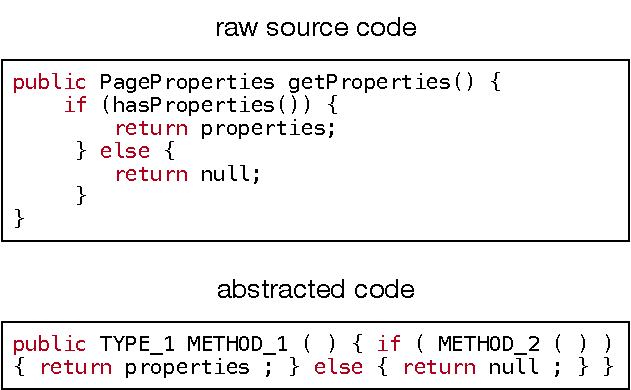
\includegraphics[width=0.37\linewidth]{eg_abs}
	\caption{Example of abstraction.}
	\label{fig:abstraction}
	\vspace{-0.1cm}
\end{figure}

The model was evaluated using quantitative metrics and qualitative analysis:
\begin{enumerate}
	\item Number of perfect predictions: prediction is considered ``perfect'' if the
	      generated revised code is identical to the expected code written.
	\item BLEU-4 score: measures the overlap between the model's output and the reference
	      revised code at the n-gram level (up to 4-grams).
	\item Levenshtein Distance: the minimum number of token edits (insertions, deletions,
	      or substitutions) needed to transform the model's output into the reference
	      code.
\end{enumerate}

%The results reveal that the reviewers comment helped a lot the model's accuracy,
%offering a $4\times$ improvement for a beam size equal to 1 (considering the
%only the token with the highest probability) and a $2\times$ for a beam size of
%10 (considering the top-10 tokens). The 2-encoder model (the one considering
%both the submitted code and the reviewers comment) had a 30\% accuracy on the
%perfect predictions, with an average of 0.91 BLEU-4 score and 0.09 Levenshtein
%distance over all the predictions.

The results reveal that the reviewers comment helped a lot the model's
accuracy, offering a $4\times$ improvement when considering the only prediction
with highest probability and a $2\times$ improvement when considering the
top-10 predictions, compared to the model receiving no reviewers' feedback in
input.

% This model obtained a 30\% accuracy on the perfect predictions, with an average
% of 0.91 BLEU-4 score and 0.09 Levenshtein distance over all the predictions.

Patanamon \etal \cite{patanamon:icse2022} and Tufano \etal
\cite{tufano:icse2022} showed that using more advanced techniques such as
Byte-Pair Encoding and transformer models can substantially enhances the
automation of this task.

%Neural Machine Translation significantly enhances performance, addressing
%challenges with out-of-vocabulary terms and large vocabulary sizes.
%Additionally,  showed that using the
%Text-To-Text Transfer Transformer (T5) model can also effectively support the
%code review process, particularly for tasks involving code revision.

\subsubsection{Code Quality Check}

Under the task of ``code quality checks'' we can factor a variety of methods
aimed at partially automating the assessment of code quality during reviews.
Researchers have developed different approaches to evaluate the quality of code
changes, although these approaches vary widely in terms of complexity and
scope.

One common approach in this area is \textit{Predicting Code Defectiveness},
which focuses on identifying potential bugs within code changes. For example,
Sharma \etal explored methods to predict whether a given code change may
introduce defects \cite{sharma:spe2019}. Similarly, Soltanifar \textit{et al.}
applied different classical machine learning techniques, such as Logistic
Regression, Naive Bayes, and Bayesian Networks, to this task, concluding that
Bayesian Networks achieved the best performance with 76\% accuracy in
predicting defectiveness \cite{soltanifar:esem2016}.

Another area of focus is \textit{Identifying Clone Refactoring Opportunities}.
Chen \etal proposed Pattern-based Clone Refactoring Inspection (PRI), a
technique that leverages refactoring pattern templates to identify clone
refactoring opportunities with high accuracy. PRI achieved 94.1\% accuracy in
identifying clone refactorings and 98.4\% in detecting inconsistencies within
these refactorings \cite{chen:compsac2017}. Additionally, Jiantao \textit{et
	al.} developed a tool aimed at checking consistency in design patterns, which
further supports refactoring efforts \cite{he:sere2013}.

In \textit{Predicting Problematic Code Lines}, researchers focus on identifying
specific lines in code that may be error-prone, to improve the review process
by flagging these lines early. Hong \etal developed a tool using machine
learning techniques to predict problematic code lines, achieving a Top-10
Accuracy of 81\% and 93\% for different scenarios. This approach allows
reviewers to concentrate on potentially problematic lines first, making the
review process more efficient.

Some researchers focused on \textit{Reviewing via Static Analysis}, applying
static analysis tools to detect issues such as code formatting violations or
potential errors. For instance, Balachandran \etal applied static analysis to
generate review comments, and Markovtsev \etal developed methods to suggest
fixes for code formatting violations, further automating quality checks during
code reviews \cite{balachandran:icse2013,markovtsev:msr2019}.

Finally, a recent trend involves \textit{Generating Review Comments} using deep
learning models to provide natural language feedback on code patches,
simulating human reviewer comments. These models are trained on large datasets
of prior code reviews and changes, allowing them to generate relevant comments
for new changes. We discuss in details the main papers addressing this task in
the following.

\paragraph{Using Pre-Trained Models to Boost Code Review Automation}

In 2022, Tufano \etal~\cite{tufano:icse2022} overcome the limitations discussed
in Section \ref{sub:revised} about their previous work \cite{tufano:icse2021}
by leveraging a pre-trained \textit{Text-to-Text Transfer Transformer} (T5)
model~\cite{raffel:jmlr2019}. Unlike previous approaches, the T5 model works
directly with raw source code without the need for code abstraction, thus
supporting more complex review. This is achieved by training T5 on a
substantially larger dataset that include a variety of realistic code review
transformations, including those requiring the introduction of new identifiers
and literals.

Empirical results show that the T5 model significantly outperforms the authors'
earlier deep learning models, particularly in scenarios involving complex code
changes. The study highlights the role of pre-training in enhancing
performance, especially in tasks involving natural language, such as generating
or interpreting comments.

However, while this approach marks a substantial improvement, the authors
acknowledge that current performance levels do not yet make T5 suitable for
deployment in real-world code review processes. They suggest that future works
should focus on increasing the accuracy of predictions, possibly by integrating
confidence-based filtering to prioritize high-quality recommendations and
combining various representations of code.

The T5 model was pre-trained on a refined corpus made from a cleaned and
filtered version of the official Stack Overflow Dump \cite{so_dump} and
CodeSearchNet \cite{Java:CodeSearchNet}. It was comprised 1,485,326 instances
of technical English, only related to Java code, and was used for pre-training
via masked token prediction.

For fine-tuning, the model used a dataset of 167,799 triplets from Java
open-source projects on GitHub and Gerrit. The dataset is of the same form as
the one from their previous work \cite{tufano:icse2021} discussed in
Section~\ref{sub:revised}, but without the abstraction process.

The model evaluation was conducted on a dataset of 16,780 instances. The
primary metric was "perfect predictions," meaning cases where the model’s
output exactly matched the expected output of the specified tasks. They also
used the BLEU (Bilingual Evaluation Understudy) score \cite{papineni2002bleu}
to evaluate the similarity between the generated review and the expected one,
however it didn't turn out to be very useful, given the low number of perfect
matches.

The authors also conducted a more in-depth analysis by examining 100 instances
where the model predictions did not achieve a perfect match with the target
output in the triplet. For the code-to-comment task, 36 instances were found to
be semantically equivalent, and 10 were alternative solutions. This analysis
indicates that perfect matches represent only a lower bound of the model's
potential performance, as many predictions classified as "wrong" were in fact
correct but formulated differently.

\paragraph{CommentFinder: A Simpler, Faster, More Accurate Code Review Comments Recommendation}

Hong \emph{et al.} \cite{hong:esecfse2022} introduced CommentFinder, a
retrieval-based approach to recommending code review comments for software
development. The approach addresses limitations in prior deep learning
(DL)-based methods \cite{tufano:icse2022}, which, while promising, are
computationally expensive and resource-intensive. CommentFinder uses
information retrieval techniques to recommend comments by finding similarities
between code changes and their associated review comments in a pre-existing
dataset, significantly reducing computational demands and time.

CommentFinder operates in three primary steps: vectorizing code changes using a
Bag-of-Words model, retrieving the most similar methods based on cosine
distance, and refining the results with Gestalt Pattern Matching (GPM) to
recommend the most relevant comments. This process eliminates the need for a
training phase, distinguishing it from the DL-based approaches that require
substantial computational resources for training.

The tool has been trained on the same dataset as the one from Tufano \textit{et
	al.} \cite{tufano:icse2022} and uses the same evaluation methods. CommentFinder
outperformed the DL approach, achieving 32\%-51\% higher perfect predictions
and 3\%-28\% higher BLEU scores. Additionally, CommentFinder was 49 times
faster in computational time, taking only 4 minutes compared to 194 minutes for
the DL model.

\paragraph{AUGER: Automatically Generating Review Comments with Pre-training Models}

Li \emph{et al.} \cite{li.l:esecfse2022} introduced AUGER, a review generator
similar to what Tufano \etal has done \cite{tufano:icse2022}, since it uses a
T5 model, but on a coarser level, as it aims to focus on review lines instead
of functions.

The dataset used to train AUGER comprises 10,882 code changes extracted from 11
influential Java projects on GitHub, amounting to 79,344 manually curated
review comments. The authors employ extensive preprocessing, including semantic
augmentation and heuristic filtering, to ensure the dataset's quality. The
training process incorporates fine-tuning the T5 model to understand
correlations between code changes and their respective review comments. This
approach allows for the generation of comments tailored to specific lines of
code rather than broader functional segments.

To evaluate AUGER, the authors conduct experiments using metrics such as
ROUGE-L and perfect prediction rates. AUGER outperforms baseline models,
achieving a 37.38\% improvement in ROUGE-L over traditional methods, such as
LSTM and CodeBERT. Additionally, case studies demonstrate that 29\% of its
generated comments are rated as useful, aligning closely with human reviewer
performance. The model's ability to generate comments in under 20 seconds
highlights its practical efficiency compared to manual review.

\paragraph{Automating Code Review Activities by Large-Scale Pre-training}

Li \emph{et al.} \cite{li.l:esecfse2022} introduced CodeReviewer, a pre-trained
encoder-decoder model specifically designed for automating key aspects of the
code review process. This includes tasks such as code change quality
estimation, review comment generation, and code refinement. The model builds on
a transformer-based architecture, leveraging advancements in large-scale
pre-training to tackle the complexity of code review tasks effectively.

CodeReviewer was trained on a novel dataset constructed from GitHub pull
requests, covering code changes and their corresponding review comments across
nine popular programming languages (C, C++, C\#, Go, Java, JavaScript, PHP,
Python and Ruby). In total, the dataset consists of approximately 7.9 million
pull requests from 1,161 high-quality repositories. This multilingual dataset
is not only extensive but also meticulously curated to ensure high-quality data
for both pre-training and downstream evaluation. To have a more effective
pre-training process, it was divided into four steps: diff tag prediction,
denoising code diff, denoising review comments, and review comment generation.
This was made to enhance the model's capacity to understand and interact with the
unique structures of code diffs and reviews. The dataset formation involved
extensive preprocessing to align code changes with corresponding review
comments. Code changes were represented using the "diff hunk" format, which
highlights added, deleted, and unchanged lines, making the dataset particularly
suitable for the code review scenario. Comments authored by the contributors
themselves were excluded to focus solely on reviewer input. To enhance the
relevance of the code refinement dataset, triplets of (original code, review
comment, revised code) were extracted from commits, ensuring that the model
could learn from meaningful revisions influenced by reviewer feedback.

The evaluation benchmarks demonstrated that CodeReviewer consistently
outperformed state-of-the-art models in all three targeted tasks. For code
change quality estimation, the model exhibited superior precision and F1
scores, reflecting its ability to effectively prioritize potentially
problematic code segments. In review comment generation, CodeReviewer produced
comments with higher informativeness and relevance scores compared to its
competitors, as validated through both automated metrics and human evaluation.
Similarly, in the code refinement task, it achieved a notable increase in BLEU
scores and perfect prediction rates, showcasing its ability to assist
developers in implementing reviewer feedback accurately.

\subsubsection{Assessing Review Quality}

While previous research has primarily focused on assisting the review process
by providing reviewers with additional information or reducing their workload,
studies in this area aim to evaluate the quality of the reviews themselves.
This line of research seeks to give feedback to reviewers, allowing them to
improve the effectiveness of their comments and suggestions where necessary.

% NOTE: this might be useful for us to determine which reviews are useful,
% especially what Pangsakulyanont did (?) and maybe also Rahman
One approach in this area involves \textit{Classifying the Usefulness of Review
	Comments}, which determines whether a review comment is helpful to the
contributor. Hasan \etal \cite{hasan:emse2021} investigated this classification
in an industrial setting, while Pangsakulyanont \textit{et
	al.}\cite{pangsakulyanont:iwesep2014} explored similar techniques within
open-source software environments. Additionally, Rahman \etal
\cite{rahman:msr2017} developed a prediction model called RevHelper to assess
comment usefulness, testing it on a dataset of 1,482 reviews and achieving an
accuracy of 66\% in predicting whether a review comment would be useful.

Another related task is \textit{Identifying Review Comments Needing Further
	Explanations}, which focuses on identifying comments that may be unclear and
thus require more detail to be fully understood by the contributor. Rahman
\etal \cite{rahman:esem2022} addressed this challenge by analyzing review
comments that lacked sufficient context, allowing contributors to take specific
action for clarification.

\subsubsection{Code Review Sentiment Analysis}

During the code review process, a developer (reviewer) may provide critiques
directed at a peer (contributor). The way these critiques are expressed in the
reviewer’s comments can significantly impact the success of the entire review
process. To support this, researchers have applied sentiment analysis
techniques to automatically classify the tone of reviewers' comments
\cite{ahmed:ase2017}: Flagging comments with negative sentiments offers
valuable feedback to reviewers, allowing them to reconsider potentially
problematic remarks. Similarly, Egelman \etal \cite{egelman:icse2020} focus on
identifying a specific subset of negative comments, \ie those that suggest a
reviewer’s intent to block a change request due to interpersonal conflicts
rather than issues with the quality of the submitted code.

\subsubsection{Retrieval of Similar Code Reviews/Code Changes}
Retrieval techniques have been applied to create recommender systems that
support code review in various ways. For example, when a code fragment is up
for review, some methods \cite{guo2020review,gupta:sigkdd2018,siow:saner2020}
pull up past reviews of similar code fragments and suggest reusable comments to
the reviewer, as these comments were previously used to recommend improvements
for similar code. Rahman \etal \cite{rahman:esem2022} proposed a similar
approach, but with a focus on helping the contributor by providing examples of
reviews similar to the feedback they’re receiving, which can help them better
understand the reviewer’s suggestions. On the other hand, Ueda \etal
\cite{ueda:iwsc2019} concentrated on identifying common improvement patterns in
code reviews—frequent changes that reviewers recommend. These patterns could
potentially be applied to enhance the code quality even before the review
begins.

\subsubsection{Time Management}
Research shows that both open-source and industrial projects can involve
hundreds of reviews each month. In such a high-volume environment, managing
time efficiently is crucial, and researchers have proposed solutions to help
allocate reviewers’ time more effectively. Unlike previous techniques focused
on automating specific review tasks, these approaches aim to enhance the
information available to reviewers and managers, potentially leading to better
decision-making in the review process.

Some of these solutions can be combined into a pipeline to streamline code
review. For instance, methods for predicting the time needed to complete a pull
request \cite{maddila:esefse2019,shan:esecfse2022} make it possible to identify
overdue requests \cite{shan:esecfse2022}, meaning those taking longer than
anticipated. These flagged pull requests can then be analyzed using techniques
that identify the "blocking actor(s)" \cite{shan:esecfse2022}—individuals
responsible for the delay—enabling teams to either prompt action or, if
feasible, reassign the task.

\subsection{Benchmarks to Assess DL-based Solutions for Code-related Tasks}

Table~\ref{tab:benchs} provides an overview of key benchmarks designed to
evaluate DL-based solutions for various code-related tasks, including code
generation, code editing, and multitask capabilities. The table categorizes
these benchmarks by task type, release year, dataset size, and supported
programming languages. These benchmarks serve as critical tools for assessing
the performance and practicality of DL models in software engineering contexts.
We will delve into the specifics of each benchmark to better understand their
design, scope, and significance.

\begin{table}[ht]
	\centering
	\begin{tabular}{llrrl}
		\toprule
		\textbf{Category}     &
		\textbf{Name}         &
		\textbf{Release}      &
		\textbf{\# instances} &
		\textbf{Languages}                                                                                              \\
		\midrule
		Code Generation       & HumanEval \cite{chen2021}                     & 2021 & 164       & Python               \\
		                      & MultiPL-E \cite{cassano2022}                  & 2023 & 164       & 18 languages         \\
		                      & CoderEval \cite{Zhang_2024}                   & 2024 & 230 + 230 & Python + Java        \\
		\arrayrulecolor{lightgray}\hline
		Code Editing          & SWE-bench \cite{jimenez2024swebench}          & 2024 & 2,294     & Python               \\
		                      & DebugBench \cite{tian2024debugbench}          & 2024 & 4,253     & C++, Java and Python \\
		                      & CodeEditorBench \cite{guo2024codeeditorbench} & 2024 & 7,961     & C++, Java and Python \\
		\arrayrulecolor{lightgray}\hline
		Multitask             & CoderUJB \cite{zeng2024coderujb}              & 2024 & 2,239     & Java                 \\
		\arrayrulecolor{black}\bottomrule
	\end{tabular}
	\caption{Benchmarks to Assess DL-based Solutions for Code-related Tasks}\label{tab:benchs}
\end{table}

\subsubsection{Code generation}

\paragraph{HumanEval \cite{chen2021}}
HumanEval is used to measure functional correctness for synthesizing programs from
docstrings. It consists of 164 original programming problems, assessing
language comprehension, algorithms, and simple mathematics, with some
comparable to simple software interview questions.

\paragraph{MultiPL-E \cite{cassano2022}}
MultiPL-E is a multi-programming language benchmark for evaluating the code
generation performance of large language model (LLMs) of code. It expands on
the previous benchmark by translating the problems into 18 different
programming languages.

\paragraph{CoderEval \cite{Zhang_2024}}
CoderEval is a code generation benchmark to evaluate the performance
of generative pre-trained models. Compared with the widely-used HumanEval
benchmark from OpenAI, CoderEval can be used to evaluate the performance of
models against pragmatic code generation beyond just generating standalone
functions. It is comprised 230 functions from 43 Python projects and 230 methods
from 10 Java projects. For each function/method, the authors extracted the original
docstring/comment, the signature, the code implementation, and the corresponding
test code (if exists) to form one function-level code generation task. CoderEval
can be viewed as a superset of HumanEval.

\subsubsection{Code editing}

\paragraph{SWE-bench \cite{jimenez2024swebench}}
SWE-Bench is a benchmark designed to evaluate the capabilities of language
models in addressing real-world software engineering problems sourced from
GitHub. It comprises 2,294 tasks derived from issues and pull requests in 12
popular Python repositories. These tasks require models to edit large and
complex codebases to resolve bugs or implement new features, often demanding
context comprehension across multiple files, execution environment interaction,
and sophisticated reasoning. Solutions are evaluated using repository-specific
tests, with success measured by the resolution of predefined "fail-to-pass"
tests. Despite its rigor, state-of-the-art models show limited performance,
highlighting SWE-Bench's value as a challenging benchmark for advancing language
models' practical software engineering capabilities.

\paragraph{DebugBench \cite{tian2024debugbench}}
DebugBench is a benchmark designed to evaluate the debugging capabilities of
large language models (LLMs) through 4,253 instances of buggy code. Covering
three programming languages: C++, Java, and Python. DebugBench categorizes bugs
into four major groups (Syntax, Reference, Logic, and Multiple errors) and 18
subtypes. The dataset is derived from code snippets on LeetCode and enhanced
with synthetic bugs implanted by GPT-4. Rigorous filtering and manual
inspections ensure the integrity and diversity of the dataset. Evaluations
using both closed-source and open-source LLMs reveal significant gaps in
debugging performance compared to humans, especially for logic and multiple
errors. DebugBench highlights the potential for runtime feedback and its
varying effects across bug types, providing a robust platform for advancing LLM
debugging capabilities.

\paragraph{CodeEditorBench \cite{guo2024codeeditorbench}}
CodeEditorBench is a benchmark designed to assess the code editing capabilities
of LLMs across four key tasks: debugging, translating,
polishing, and requirement switching. It incorporates a dataset of 7,961 tasks
derived from sources such as LeetCode and CodeNet, enriched with test cases
generated by LLMs and validated by an online judge system. Evaluations of 19
LLMs reveal significant performance disparities, with closed-source models like
GPT-4 excelling in debugging and translating, while challenges persist in
polishing and requirement adaptation tasks.

\subsubsection{Multitask}

\paragraph{CoderUJB \cite{zeng2024coderujb}}
CoderUJB is a comprehensive benchmark tailored to evaluate the programming
capabilities of LLMs in realistic Java-based development
scenarios. Built from 17 open-source Java projects, it comprises 2,239
programming tasks spanning five areas: functional code generation, code-based
test generation, issue-based test generation, defect detection, and automated
program repair. Each task is executable and evaluated within a complete project
context, reflecting real-world software engineering challenges. The benchmark
also assesses the impact of pre-training and instruction fine-tuning on LLM
performance, revealing gaps in handling non-functional code tasks like defect
detection.

\subsection{Summing up}

Our benchmark introduces two key innovations compared to the previously
discussed benchmarks. First, there are currently no benchmarks explicitly
designed to evaluate the generation of code review comments. Second, none of
the existing benchmarks, even those about code editing, exercise models in the
task of addressing a given code review comment expressed in natural language.
Our objective is to assess the quality of generated code by considering both
the submitted code and the accompanying reviewer's comments.

We expect the proposed benchmark to substantially increase the reliability of
empirical evaluations performed on deep learning-based code review automation
tools.

% !TEX root = ../main.tex
\section{CRAB: Code Review Automated Benchmark}

\subsection{Overview}

In this section, we describe the construction of a high-quality Java-only dataset of code-review
triplets. Each triplet comprises three elements: the code snapshot before the review, the natural
language review comment and the revised code after that change has been applied. Our work supports
two complementary benchmarks: the first is review comment generation, asks a model to predict the
review comment given the pre-review code; the second is code refinement, a strict subset of the
first, asks a model to generate the revised code that implements the suggestion.


We focused on Java projects and aimed for high quality over quantity. That means we only kept
examples that are self-contained, testable, and likely to be meaningful. As a starting point, we
used the \textit{GHS} dataset and tool introduced by Dabić \etal~\cite{Dabic:msr2021data}, which
supports project sampling for Mining Software Repositories (MSR) studies by providing rich metadata
for over 700'000 GitHub repositories. Their platform made it possible to filter for Java
repositories with relevant properties like number of commits, license, and recent activity.

This section explains how we constructed the dataset, how we defined the two benchmark tasks
(comment generation and code refinement), and how we filtered and validated the data to ensure it’s
useful for evaluating future models.


\subsection{Data Source}

\subsubsection{Repository Sampling}

We began by querying the \textit{GHS} dataset~\cite{Dabic:msr2021data}, a large-scale repository
mining platform that indexes metadata for over 700'000 GitHub projects. Using the web interface at
\url{https://seart-ghs.si.usi.ch}, we applied two simple filters:

\begin{itemize}
	\item The repository must have had at least 100 pull requests.
	\item The date of the last commit must fall within the year 2025.
\end{itemize}

These criteria ensured that we targeted active, collaborative projects likely to have meaningful
code review activity. We exported the matching repository list in CSV format and used it as input
for our processing pipeline.

We applied minimal filtering beyond that. A small number of repositories were manually excluded
during processing, mostly due to extreme build times or authentication issues.

\subsubsection{Pull Request Selection}

For each selected repository, we searched for pull requests that reflect a clean and minimal review
interaction. Specifically, we looked for PRs that:

\begin{itemize}
	\item Were successfully merged into the main branch.
	\item Contain either one review comment or two, where the second is a reply from the PR author.
\end{itemize}

The goal is to capture cases where a reviewer leaves a single comment and the author either does not
respond in writing, or replies directly within the thread — which we interpret as an acknowledgment
of the feedback. This keeps the setup simple and avoids ambiguous review discussions.

We made this design choice because we realized early on that it would be difficult to create clean
triplets from pull requests with multiple comments. While we can always locate where each comment
appears in the code, it's much harder to untangle which subsequent code changes correspond to which
comment in an automatic way. This makes it challenging to extract multiple, independent \subCode,
\revComment and \revCode triplets from a single pull request. By focusing on PRs with only one
comment (plus an optional reply), we ensure that each PR maps to a single, self-contained instance.
This keeps the data interpretable and makes the benchmark more reliable.

Of course, even in these single-comment PRs, not all follow-up commits are guaranteed to directly
address the reviewer’s feedback. We handle these exceptions through manual validation, as detailed
later in Section~\ref{sec:manual-selection}.

\subsection{Automated Extraction Pipeline}
\label{sec:pipeline}
Transforming raw pull requests into usable training examples requires more than just scraping
metadata from GitHub. It involves carefully extracting code changes, associating them with reviewer
comments, validating their build and testability, and preserving the relevant context along the way.
To achieve this at scale and with high fidelity, we developed a robust, modular, and fully automated
pipeline. This system processes each pull request independently, performing all necessary
extraction, validation, and archival steps in a reproducible and fault-tolerant manner.

The following sections describe the guiding principles behind the pipeline, its overall
architecture, the key stages involved, and the mechanisms used for error handling and parallel
execution.

\subsubsection{Purpose and Design Philosophy}

The goal of the automated extraction pipeline is to transform raw pull requests from open-source
repositories into structured, high-quality dataset entries suitable for evaluation. To do this
effectively, the system must perform a complex sequence of steps, ranging from low-level repository
operations to high-level semantic filtering, while maintaining reliability, traceability, and
consistency at scale.

This pipeline is designed to be fully automated. Given a set of candidate repositories, it processes
each pull request independently from end to end, requiring no human intervention during execution.
This level of automation is critical for large-scale dataset construction, but it comes with
challenges: repositories vary widely in structure, quality, and tooling, and small inconsistencies
can derail processing unless handled robustly.

To address this, the pipeline is built with three guiding principles:
\begin{enumerate}
	\item \textbf{Isolation and Reproducibility.} All build and test steps are executed inside
	      Docker containers, ensuring that the results are not affected by the host system and can
	      be reproduced reliably.

	\item \textbf{Resilience to Failure.} Each processing step is isolated and allowed to fail
	      independently. A failure in one phase, such as test execution or coverage extraction, does
	      not invalidate the rest of the data. Instead, failures are captured and logged with
	      structured metadata so that partial but useful entries can still be retained.

	\item \textbf{Transparency and Debuggability.} Every step records its outcome and, in the case
	      of failure, the exact reason. This enables downstream analysis of failure rates and causes,
	      and facilitates future improvements to the pipeline itself.
\end{enumerate}

The result is a system capable of ingesting a wide variety of pull requests, gracefully handling
both clean and noisy cases, and producing a structured dataset where each entry includes not only
the final output but also a trace of what succeeded or failed during processing.

\subsubsection{High-Level Architecture}

The pipeline is structured as a sequential series of processing stages, each responsible for a
well-defined operation on a single pull request. These stages are executed one after the other, and
at each step, relevant metadata is recorded and potential errors are caught and stored. This design
promotes clarity, modularity, and traceability throughout the entire process.

At a high level, the pipeline begins by cloning the repository and extracting the relevant code and
comment information from the pull request. It then checks out the code states at the beginning and
end of the pull request, archives these snapshots, and determines whether the comment pertains to
code. If so, the pipeline continues by identifying the build system, attempting to compile the
project, executing the test suite, and extracting coverage metrics. Regardless of success or failure
in any step, a dataset entry is created and tagged with its processing outcome.

Although each pull request is treated independently from a logical standpoint, in practice, the
underlying repository state is shared on disk. For reasons of disk space efficiency, we do not
duplicate the repository for each pull request. As a result, pull requests from the same repository
are processed sequentially to avoid race conditions and state conflicts. However, because
repositories themselves are fully independent, the pipeline is parallelized at the repository level:
different repositories can be processed concurrently without interference. This strategy balances
isolation with scalability, allowing the system to make efficient use of compute resources while
maintaining correctness.

Figure~\ref{fig:pipeline} presents a simplified overview of the pipeline’s control flow. The diagram
groups the processing steps into three main phases: \textit{Setup}, \textit{Build \& Validation
	Assessment}, and \textit{Finalization}. There is also a decision point between \textit{Setup} and
\textit{Build \& Validation Assessment} that short-circuits unnecessary work when the comment is not
related to code.

\begin{itemize}
	\item \textbf{Setup}: This phase includes cloning the repository, extracting the diffs and
	      modified files, capturing the review comment, and archiving the relevant commits to preserve
	      a reproducible view of the pull request before and after the review.

	\item \textbf{Eligibility Check}: Before performing more expensive operations, the pipeline
	      checks whether the comment targets a Java file. If it does not, the system skips the
	      build phase entirely and proceeds directly to finalization, as test and build analysis
	      are not relevant.

	\item \textbf{Build \& Test Assessment}: For code-related comments, the pipeline identifies the build system,
	      attempts to compile the code, runs the test suite, and tries to generate code coverage using
	      JaCoCo. These steps are executed inside Docker containers for reproducibility.

	\item \textbf{Finalization}: Regardless of success or failure in the previous phases, the
	      pipeline saves the dataset entry along with rich metadata describing the processing outcome,
	      including reasons for failure when applicable.
\end{itemize}

This structure ensures a clean separation of concerns while maintaining extensibility and fault
tolerance. New capabilities or heuristics can be integrated into any phase with minimal disruption
to the rest of the system. The modular layout also enables robust error handling, allowing the
pipeline to continue processing even when individual pull requests encounter issues. This makes the
system scalable and resilient when applied to large and diverse sets of repositories.

\begin{figure}[!htbp]
	\centering
	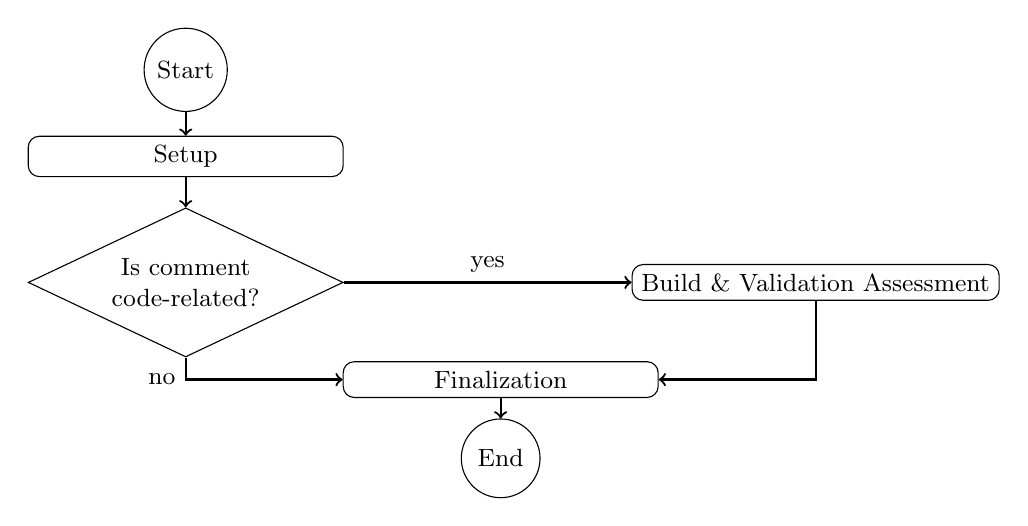
\begin{tikzpicture}[
			node distance=1cm and 1cm,
			every node/.style={font=\small},
			startstop/.style={circle, draw, minimum size=1cm},
			process/.style={rectangle, draw, rounded corners, minimum width=4cm},
			decision/.style={diamond, draw, minimum width = 4cm, aspect = 2, align=center},
			arrow/.style={->, thick}
		]

		\node (start) [startstop] {Start};
		\node (prep) [process, below of=start, yshift=-.1cm] {Setup};
		\node (iscode) [decision, below of=prep, yshift=-.6cm] {Is comment\\code-related?};
		\node (validation) [process, right of=iscode, xshift=7cm] {Build \& Validation Assessment};
		\coordinate (mid) at ($ (iscode)!0.5!(validation) $);
		\node (save) [process] at ($(mid |- validation.south)+(0,-1cm)$) {Finalization};
		\node (end) [startstop, below of = save] {End};

		% arrows - linear path
		\draw[arrow] (start) -- (prep);
		\draw[arrow] (prep) -- (iscode);
		\draw[arrow] (iscode) -- node [above] {yes} (validation) ;
		\draw[arrow] (iscode) |- node [left] {no}(save) ;
		\draw[arrow] (validation) |- (save);
		\draw[arrow] (save) -- (end);
	\end{tikzpicture}
	\caption{Automated pipeline for processing a single pull request.}
	\label{fig:pipeline}
\end{figure}

\subsubsection{Key Pipeline Stages}

This section provides a more detailed walkthrough of the core stages outlined in
Figure~\ref{fig:pipeline}. Each pull request passes through the same structured sequence of
operations, with intermediate state and outcomes logged to facilitate inspection, debugging, and
dataset filtering.

\paragraph{Setup.} The pipeline begins by cloning the target repository, unless it already exists
locally. To avoid unnecessary downloads and to support resuming interrupted runs, previously cloned
repositories are reused. Once the repository is available, the system retrieves both the base and
merged commits of the pull request. These two commits serve as reference points to extract the code
diffs before and after the review comment.

The system then attempts to extract the content of all files modified by the pull request. This is
done using the GitHub API when possible, and directly from disk as a fallback when the API is
incomplete or fails to deliver consistent results. Special care is taken to record both the pre- and
post-merge versions of each file, as well as to ensure coverage data can be attached to the correct
source snapshot.

Review comments are extracted and filtered to retain only those that reference a specific file and
line range. This is necessary because GitHub occasionally serves comments without reliable line
anchoring. Comments without a valid line mapping are discarded early
in the process to reduce ambiguity downstream.

Both the base and merged states of the repository are archived in compressed form. These serve
distinct purposes. The base state (representing the code before any changes introduced by the pull
request) is primarily stored to provide broader context to models that may benefit from
access to the entire project structure. While the dataset already includes the full content of the
specific files involved in the pull request, some models may require a more holistic view of the
repository to make informed predictions. The merged state, on the other hand, is preserved for
evaluation purposes. In particular, it is used to test model-generated submissions in the context of
the code refinement task. Details of this evaluation setup are discussed further in
Section~\ref{sec:refinement}.

\paragraph{Eligibility Check.} Once the setup phase is complete, the system performs a quick check
to determine whether the review comment is attached to a source code file. If the comment points to
a non-code file (e.g. documentation, configuration files, or assets) it is extremely unlikely that
the suggested change involves actual code behavior. In such cases, running the full build phase,
that includes build, test, and coverage analysis, would be unnecessary and wasteful. To conserve
computational resources and reduce processing time, the pipeline bypasses that phase entirely for
these entries and moves directly to finalization. This early filtering mechanism ensures that only
potentially meaningful code-related changes undergo the more expensive analysis.

\paragraph{Build \& Test Assessment.} For comments that do target Java files, the pipeline enters
the build and test assessment phase. It first detects whether the repository uses Maven or Gradle by
inspecting known build configuration files. This allows it to spin up the appropriate Docker
container, preconfigured with the necessary environment for building and testing Java code.

Once inside the container, the pipeline attempts to compile the codebase. If the build succeeds, it
proceeds to run the test suite. If tests are detected and executed successfully, the system then
attempts to extract code coverage information using JaCoCo. If the project already includes JaCoCo
in its configuration, the system leverages that setup directly. Otherwise, it attempts to inject the
required configuration into the build process. While this injection is not guaranteed to succeed in
all cases, it enables coverage reporting in many repositories that would otherwise lack it.

After coverage reports are generated, the system analyzes them to determine whether the file
affected by the review comment is included in the results. This is done by extracting the fully
qualified class name from the file and searching for it in the coverage data. Due to the presence of
multi-module repositories and inconsistent directory structures, this association is not always
perfect. As discussed in Section~\ref{sec:multi-project-repo}, users must sometimes manually verify
that the reported coverage corresponds to the correct subproject.

\paragraph{Finalization.} At the end of the pipeline, the system records the outcome of each
processing step, including whether the pull request built and tested successfully, whether the
commented file was covered by tests, and whether the comment was code-related. If any step failed,
the reason is logged in structured metadata using a dedicated exception hierarchy. This allows for
filtering and debugging later on.

Every processed pull request results in a dataset entry, even if a phase failed. This is a
deliberate design choice: entries that fail the build phase may still contain useful review comments
for tasks such as comment generation. By capturing the full trace of each pull request—including
what succeeded, what failed, and why—the pipeline produces a dataset that is not only rich in
content but also transparent and debuggable.

\subsubsection{Failure Handling and Debuggability}

One of the key challenges in building a dataset from real-world repositories is handling the wide
range of inconsistencies, misconfigurations, and unexpected edge cases that arise in practice.
Repositories may have incomplete histories, broken builds, missing dependencies, or improperly
formatted comments. Rather than treat these cases as exceptions to be discarded, the pipeline is
designed to process them as first-class outcomes and record their failure modes explicitly.

Each stage of the pipeline is wrapped in fine-grained error handling logic. When a step fails
(whether due to a Git error, an unresolvable build issue, or malformed metadata) the failure is
caught, and a dedicated custom exception class is raised. These exceptions are structured,
categorized, and logged in the metadata of the corresponding dataset entry. This approach allows
each pull request to contribute useful diagnostic information, even when it does not yield a fully
valid instance.

This design serves two purposes. First, it enables comprehensive statistics about failure rates and
patterns across repositories. For example, one can measure how many entries fail at the build step,
how many fail due to missing line mappings in comments, or how often coverage extraction fails due
to JaCoCo injection issues. These insights help guide improvements to the pipeline and provide a
realistic picture of what can be expected when operating at scale.

Second, by retaining partially processed entries and clearly tagging them with their failure
context, the pipeline supports debugging, validation, and experimentation without requiring
re-processing from scratch. Entries that fail the build phase may still contain valuable
content for the comment generation task.

This robust failure management strategy ensures that the pipeline remains resilient in the face of
the inconsistencies inherent to open-source codebases. It allows for high-throughput processing
without sacrificing visibility into what went wrong, and it provides a mechanism for iterative
refinement over time.

\subsubsection{Parallelism and Scalability}

To process a large number of repositories efficiently, the pipeline is designed with parallel
execution capabilities. However, parallelism is applied at the repository level rather than the pull
request level. This distinction is critical due to the way repositories are managed on disk.

During processing, the build, test, and coverage phases operate directly on a local clone of the
repository. Creating separate copies of the repository for each pull request would incur a
substantial disk overhead, especially for large projects. To avoid this, the pipeline reuses a
single local clone per repository. This means that only one pull request per repository can be
processed at a time, ensuring consistency and preventing conflicts caused by concurrent checkouts or
file modifications.

To scale across repositories, the pipeline uses a multi-process architecture where multiple worker
processes handle different repositories in parallel. Each worker runs its own isolated pipeline
instance, with no shared state, and processes one repository at a time. This approach makes full use
of available compute resources while preserving correctness and reproducibility.

Parallelism also helps avoid bottlenecks caused by unbalanced workloads. Some repositories contain
only a handful of pull requests and can be processed quickly, while others (especially those with
extensive histories and complex build steps) take significantly longer. By distributing work across
multiple repositories concurrently, the system avoids having to wait on the slowest task to proceed.

However, true scalability is limited by another important factor: GitHub’s API rate limits. These
constraints, and how the pipeline addresses them, are discussed in the next section.

\subsubsection{Dealing with API Limits and Caching}

A critical bottleneck in any large-scale GitHub data processing pipeline is the platform's API rate
limit. GitHub imposes a cap of 5000 requests per hour per authenticated user. At first glance, this
may appear generous, but in practice, it is quickly exhausted due to how the GitHub Python client
operates.

The library adopts a lazy-loading design: most objects returned from the API are incomplete by
default and only fetch their full data when specific attributes are accessed. While this is
efficient for bandwidth and memory usage, it results in many additional network calls during regular
use. A single pull request may require dozens requests to fetch metadata, commit histories,
comments and file contents.

Fortunately, the library provides automatic handling of rate limit exhaustion. When the limit is
reached, it enters a waiting state and resumes once requests become available again. This makes it
safe to run the pipeline with multiple threads or processes: each one will automatically pause and
continue as needed without crashing or violating GitHub’s usage policies.

Despite this robustness, long pauses can be impractical when running large-scale crawls. To mitigate
this, the pipeline includes two layers of caching:

\begin{itemize}
	\item \textbf{HTTP-level caching:} The GitHub responses themselves are cached locally using an
	      auxiliary Python library, allowing the pipeline to skip API calls for data that has already
	      been retrieved. This not only saves bandwidth and time but also avoids rate limits entirely
	      for cached objects.

	\item \textbf{Pipeline-level checkpointing:} The system tracks which pull requests have already
	      been processed. If the pipeline is interrupted or restarted, it can pick up where it left
	      off without reprocessing completed work. This enables stop-and-resume operation, which is
	      especially valuable for long runs or incremental dataset builds.
\end{itemize}

While the GitHub Python library lacks thorough documentation, its internal behavior, once inspected,
proves reliable and well-suited for automation at scale. On several occasions, the implementation
had to be understood by directly reading its source code. Nonetheless, once these behaviors are
accounted for, the client operates smoothly, and the pipeline is able to run unattended for extended
periods, managing its own retries and pacing.

These design decisions—automated rate limit handling, layered caching, and task
checkpointing—combine to make the pipeline not just scalable in theory, but practically usable for
large-scale, real-world dataset construction.

\subsection{Build, Test \& Coverage}


\subsubsection{Motivation and Purpose}

Ensuring that each pull request can be built, tested, and instrumented for coverage is a key step in
constructing a dataset that goes beyond static code analysis. This phase is not just a validation
step for technical completeness, it also lays the groundwork for more robust evaluation. The ability
to compile and execute the code opens up the possibility of behavior-based assessment, which is
critical when evaluating code refinement models.

In contrast to similarity-based metrics such as CodeBLEU, which penalize variations in syntax even
when semantics are preserved, test-based evaluation allows for multiple valid implementations to be
accepted as long as they do not introduce regressions. While passing tests do not guarantee the
correctness of a change, they do strongly suggest that the change is not invalid. Failing tests, on
the other hand, clearly indicate broken behavior. This framing enables more realistic and flexible
model evaluation, better aligned with real-world development practices.

\subsubsection{Test Detection}

The first step is to determine whether the repository contains any form of automated
testing. This is accomplished by scanning the build configuration files for known testing libraries
(e.g., JUnit, TestNG, Mockito) and build system keywords such as \path{testImplementation} or
\path{functionalTests}. In addition to static analysis of the build file, the system also
inspects conventional test directories, such as \path{src/test/java} or \path{test/}, which
frequently contain unit or integration tests. This dual approach increases the reliability of test
detection across a broad set of repository structures.

\subsubsection{Execution Environment}

To ensure reproducibility, consistency, and isolation from the host system, all compilation and test
operations are executed within Docker containers. Two container environments are maintained,
corresponding to the two supported Java build systems: Maven and Gradle. Each container includes the
necessary tools, dependencies, and environment settings to execute a typical Java project. This
ensures that the results are not affected by host-specific variations, such as Java versions, OS
configuration, or missing libraries.

The architecture is designed with extensibility in mind. Build system support is modularized so that
new systems (such as Ant or Bazel) can be integrated by adding new handler classes and corresponding
container definitions. This separation of concerns facilitates future expansion to accommodate more
diverse types of software projects. Moreover, because the interface between the build system logic
and the rest of the pipeline is language agnostic, it is hypothetically straightforward to extend
support beyond Java and handle projects written in entirely different programming languages,
provided suitable build and test tooling exists for them.

\subsubsection{Coverage Generation}

Once a repository has been successfully built and tested, the next objective is to collect code
coverage data. This is primarily done using JaCoCo, a widely adopted tool for Java coverage
reporting. If the project is already configured with JaCoCo, the system attempts to run its existing
configuration directly. If this fails, typically due to the absence of the plugin, the system attempts
to inject JaCoCo manually into the build file, modifying the configuration to include the required
setup for coverage generation.

Care is taken to preserve the integrity of the build system: the original configuration is backed up
and restored if the injection fails. When successful, the injected configuration allows for the
generation of XML coverage reports, which are then parsed to extract coverage percentages for
individual files.

\subsubsection{Handling Multi-Project Repositories}

\label{sec:multi-project-repo}
A major challenge arises when dealing with large repositories that are organized into multiple
subprojects. These may be loosely coupled, deeply nested, or follow custom directory conventions.
Because of this structural diversity, it is difficult to reliably map a given Java file to a
specific coverage report. To approximate this mapping, the system extracts the fully qualified class
name of each commented file and searches for it across all available coverage files. If found, the
file is marked as covered.

This approach, while pragmatic, is not foolproof. It does not guarantee that the coverage report
belongs to the same subproject as the file in question. Given the variability in repository layout,
automatic resolution of this ambiguity is not feasible. Users are therefore advised to manually
verify coverage associations in cases where accuracy is critical.

\subsubsection{Enabling Flexible Evaluation}

By ensuring that the code in each pull request is buildable and testable, the dataset allows for a
richer model evaluation framework. Unlike static metrics that enforce a rigid similarity standard,
test-based validation supports functional correctness. This means that a model can propose diverse
implementations in response to reviewer comments, as long as the resulting code passes all tests. In
effect, this introduces a behavior-first evaluation protocol that aligns more closely with how
developers themselves judge correctness: not by form, but by function.

In summary, this phase adds significant value to the dataset by grounding it in real, executable
code, and by enabling flexible, semantically meaningful evaluation. Despite the technical challenges
involved—such as inconsistent configurations, incomplete test setups, and structural complexity—this
approach provides a much more powerful basis for training and evaluating automated code refinement
systems.

\subsection{Manual Selection}
\label{sec:manual-selection}

While the construction of the dataset is driven by automation to ensure scale and consistency, there
remain several aspects that fundamentally depend on human judgment. One of the most important among
these is the annotation of intent and follow-through: determining whether a reviewer’s comment
suggests a change, and whether that change was subsequently implemented in the pull request.

\subsubsection{Comment Classification}
The first layer of this process involves evaluating the nature of the review comment itself. Not all
comments are meant to trigger code modifications. Many comments are purely informational, offering
optional improvements or clarifications that do not warrant actual changes. Some comments are not
directly related to the current pull request but are instead left as notes for future work. These
typically refer to changes that should be made after the branch has been merged with another one,
but which cannot be carried out within the scope of the current pull request due to technical
constraints. Others might highlight a section of code without proposing any specific action. In
order to ensure that the dataset captures meaningful reviewer-author interactions, it is necessary
to distinguish between comments that suggest actionable modifications and those that do not.

A particularly nuanced category of comments consists of those framed as questions. While at first
glance they may appear less directive than imperative statements, questions often carry implicit
suggestions. These can be roughly divided into two main types. The first are rhetorical questions,
which are generally straightforward to interpret. These tend to imply strong disapproval or an
obvious recommendation, masked in the form of a question. For example, a reviewer might write,
\textit{``Can you move this declaration down closer to where it's used?''} or \textit{``Isn't this
	redundant with the previous check?''} In most cases, the intent behind such comments is clear: they
point out something that should be removed, refactored, or reconsidered.

The second type of question-based comment is more difficult to classify. These are genuine
inquiries, often posed in good faith, reflecting uncertainty or opening a discussion. They may
express doubt about a design choice, inquire about alternative implementations, or question whether
a particular solution addresses the intended problem. For instance, a reviewer might ask,
\textit{“Would it make sense to use a stream here instead of a loop?”} or \textit{“What happens if
	this input is null?”} The challenge with these types of comments is that they can be interpreted in
multiple ways. Some reviewers may expect an immediate change, while others are simply requesting
clarification. In many cases, the boundary between suggestion and inquiry is blurry, and
classification depends on context: including the tone of the comment, the review history, and even
the norms of the repository or organization. As a result, the decision to treat such a comment as a
change suggestion often comes down to the judgment of the person performing the manual annotation.

\subsubsection{Assessing Implementation of the Change}
Once a comment is identified as suggesting a change, the next step is to verify whether the change
was actually implemented. This involves inspecting the commits made after the comment was posted and
analyzing the diffs introduced. However, this is not as straightforward as it may seem. In modern
development workflows, especially those influenced by continuous integration and continuous
deployment (CI/CD) practices, it is common for the pull request branch to be updated with changes
from another branch, such as \texttt{main} or \texttt{dev}, before it is merged. This is often done
to resolve merge conflicts, bring in recent bug fixes, or ensure compatibility with the latest
version of the codebase. While such merges are necessary from an engineering perspective, they
introduce significant noise from the point of view of dataset construction.

When another branch is merged into the pull request, it can bring in a large number of changes that
are unrelated to the comment or even to the pull request itself. As a result, the diffs that appear
after the comment may include modifications that are completely irrelevant to the interaction being
studied. This creates a challenge: how can we isolate the changes that were made in response to the
comment from the rest?


\subsubsection{Selective Diff Curation}

To address this issue, the system incorporates a manual selection step where the user is shown the
diffs produced after the comment and is asked to select which hunks (blocks of code changes) are
relevant to the comment. This allows for precise filtering of the changes and helps construct a
cleaner, more focused dataset where only the diffs that represent a response to the review comment
are preserved.

In some cases, the situation is further complicated by the proximity of changes. Even when
irrelevant changes originate from merges or unrelated commits, they may occur in the same file or
even in adjacent lines to the relevant ones. This results in hunks that contain both the actual
response to the comment and unrelated code. Because the standard diff format groups nearby changes
into a single hunk, it becomes impossible to separate them without manual intervention. To deal with
such situations, the system provides the ability to edit the hunks directly. Users can manually trim
the diff to retain only the portions that directly address the reviewer’s feedback, discarding the
unrelated ones. This kind of fine-grained control is essential for preserving the integrity and
specificity of the dataset.

By performing this dual-level manual selection — first identifying whether a comment suggests a
change, and then isolating the relevant diff hunks — the dataset maintains a high degree of
fidelity. It captures meaningful reviewer-author interactions and filters out unrelated noise
introduced by collaborative development practices. This ensures that the final data is not only
accurate but also truly representative of how developers respond to feedback during the code review
process.

\subsubsection{Manual Selection as a Design Choice}

The decision to include a manual selection step was not an afterthought, but a deliberate design
choice. Prior work has shown that fully automated dataset construction methods often introduce a
significant amount of noise—whether due to misclassified comments, ambiguous code changes, or
incidental modifications unrelated to reviewer feedback. Rather than aiming for scale at the expense
of quality, we chose to prioritize precision and relevance. By hand-picking the instances we deemed
meaningful and representative, we ensured that the dataset would reflect true reviewer-author
interactions, with clearly identifiable suggestions and corresponding responses. This curated
approach allows for more reliable evaluation of models in tasks that require nuanced understanding
of code review dynamics.

\subsection{Paraphrases generation}
\label{sec:paraphrases}

\subsection{Dataset Schema \& Serialization}

The dataset is designed to be both expressive and flexible. Each entry represents a single pull
request and contains a rich set of data capturing the code, the reviewer comments, the surrounding
context, and the repository’s response.

\subsubsection{Schema Overview}

Each entry in the dataset encapsulates multiple layers of information. At the core is the
\texttt{metadata} object, which includes identifying fields such as repository name, pull request
number, and commit hashes. It also contains metadata about the PR’s outcome, such as whether the
project built successfully, whether the file under review was covered by tests, and whether the
comment was judged to suggest a change.

The entry also stores:
\begin{itemize}
	\item The full set of \texttt{comments}, including body text, line ranges, and paraphrases.
	\item The \texttt{files} affected by the pull request, each annotated with its content before
	      and after the change, test coverage metrics, and whether it is code-related.
	\item Two sets of \texttt{diffs}: those between the opening of the PR and the reviewer comment
	      (``before''), and those occurring after the comment (``after'').
\end{itemize}

Together, these components allow for rich modeling of code review interactions over time.
Specialized views of this data, used for comment generation or code refinement tasks, can be derived
through structured filtering.

\subsubsection{Design Rationale}

The schema is built around the principle of modularity. Rather than entangling comment logic, diff
parsing, and code coverage into a flat structure, each concept is separated into its own dedicated
field or object. This makes it easy to reason about and operate on specific parts of the dataset
independently, for example, isolating all comments that suggest a change, or extracting only the
diffs related to code files.

\subsubsection{Serialization Formats}

The dataset supports several serialization modes, depending on the intended downstream task. These
include:
\begin{itemize}
	\item \texttt{full}: All fields are retained, giving a complete view of each entry.
	\item \texttt{comment\_gen}: Only includes entries where the reviewer comment suggests a change,
	      and retains just the code state and diffs before the comment. Useful to give as input to
	      a model for the comment generation task.
	\item \texttt{code\_refinement}: Filters to entries where the change was both suggested,
	      implemented and covered by tests. Includes the comment and the ``before'' diff, but omits
	      unrelated fields. Useful to give as input to a model for the code refinement task.
	\item \texttt{webapp}: A lightweight format that includes only metadata and comments, intended
	      for use in the webapp, so that it doesn't take long to load in memory.
\end{itemize}

Each mode produces a JSON file that is readable, compact, and suitable for different types of
experiments or tools. In addition, the serialization process allows for filtering out entries that
do not meet the criteria for inclusion in the dataset, such as comments that do not suggest a change
or pull requests that failed somewhere along the pipeline described in Section \ref{sec:pipeline}.
These “faulty” entries are not part of the intended dataset and are retained only as a form of
internal logging. They serve two main purposes: enabling detailed analysis of failure patterns
(e.g., identifying how many entries failed due to missing tests or broken builds), and helping
future efforts to improve the pipeline itself. The dataset, as serialized for
evaluation, is meant to consist exclusively of clean, validated entries that support the task of
comment generation or refinement.

\subsubsection{Use Case-Driven Filtering}

This flexibility allows researchers and engineers to tailor the dataset to the task at hand. For
example, a model trained to generate review comments may only require the pre-comment diff and
associated files. A refinement model, on the other hand, benefits from both the comment and the
changes made after it, with accurate annotation of whether the diff actually addressed the
suggestion.

The ability to serialize the dataset in multiple views avoids the need to rerun the full pipeline
every time a new task is proposed. It also supports experimentation and benchmarking across
different problem formulations while keeping the core data consistent.

\subsubsection{Extensibility and Programmatic Access}

Beyond serialization, the dataset class includes convenience methods for loading, filtering, and
mapping entries by ID. Internally, the logic is implemented in a way that is agnostic to language or
repository structure. This makes it easy to adapt the system to future extensions, such as
supporting other programming languages or integrating with other evaluation pipelines.

Overall, the dataset schema and its serialization logic reflect a balance between structure,
flexibility, and practical usability, ensuring that the data can evolve alongside the research it
supports.

\subsection{Phases of Dataset Curation}

The dataset construction process was performed in two phases, each with distinct strategies for
repository filtering and pull request validation.

\subsubsection{Initial Filtering and Manual Validation}

The first phase began with a list of 4'795 repositories sourced from the GHS dataset. To narrow the
scope, a pre-filtering step was applied. Each repository was cloned, and the following conditions
were checked on the most recent commit of the default branch:

\begin{itemize}
	\item The project uses a supported build system (e.g., Maven or Gradle).
	\item It compiles successfully.
	\item All tests pass.
	\item At least one test is present.
\end{itemize}

Only repositories satisfying all criteria were retained, reducing the list to 398 projects. From
these, all available PRs were extracted, yielding 1'681 PRs in total. After manually validating
whether the comments suggested changes and whether those changes were implemented, a set of 985 PRs
was finalized for the comment generation task.

A significant limitation emerged at this stage: although 22 PRs were both compilable and testable,
none of them met the required test coverage conditions. This rendered the initial dataset
insufficient for the code refinement task.

\subsubsection{Updated Construction and Expanded Dataset}

In response, the second phase re-ran the dataset construction on the full set of 4'795 repositories.
This iteration incorporated improvements to the data collection pipeline, specifically:

\begin{itemize}
	\item Coverage checks were moved to the construction stage, rather than being deferred to manual
	      filtering.
	\item A stricter coverage criterion was applied: the PR must have at least one coverage file
	      associated with the commented file, and all reported files must exhibit non-zero line
	      coverage.
\end{itemize}

These changes led to a more refined classification of pull requests valid for code refinement.
Previously, a PR was considered valid if it compiled and tested successfully, regardless of test
coverage. Now, a PR is only considered valid if it is (a) code-related, (b) builds and tests pass,
and (c) the coverage condition is satisfied.

\subsubsection{Observations}

The improvements made between the two runs significantly enhanced the reliability of the dataset
construction process. While the first run provided useful insights, such as the overall rate of PR
failures and the effectiveness of the manual filtering. It primarily served as a proving ground for
iterating on the pipeline. Despite being limited to 398 repositories, it helped validate the
extraction logic and informed adjustments to the coverage evaluation and PR validation mechanisms.

Once the pipeline was considered robust, the second run extended the process to all 4'795
repositories. This larger scope was essential to capture a broader and more diverse set of eligible
PRs, especially for the code refinement task, that depend on accurate coverage information.

Although the updated process improves coverage filtering, many PRs still fail the coverage check.
One possible way to increase the number of PRs eligible for the refinement task would be to manually
write targeted tests for cases where the code compiles and tests pass, but the changed lines are not
yet covered.

\subsection{Dataset Statistics}

This section presents statistics from both phases of dataset construction. We begin by analyzing the
dataset derived from the 398 pre-filtered repositories. This smaller-scale dataset was the only one
subjected to manual selection, given its more manageable size of 1'681 pull requests. It allows us
to examine the failure distribution across PRs and the impact of manual validation on final PR
eligibility.

We then turn to the second dataset, built from the full set of 4'795 repositories. Although no
manual filtering was applied to this version, the insights gained from the first dataset provide a
useful baseline for interpreting its structure and expected failure patterns.

\subsubsection{Initial Dataset: Pre-filtered Repositories}

Before scaling up to a broader corpus, we conducted an initial run of the dataset construction
process on a smaller, pre-filtered set of repositories. Table~\ref{tab:initial-distribution}
summarizes the outcome of this first stage. A substantial portion of the PRs (over 64\%) encountered
issues during automated processing. These ranged from compilation failures to missing commits or
broken diffs. About 27\% of the total were not code-related (i.e., the review comments did not
target source code files). The remaining slices represent entries that passed both build and test
phases, but only 4.87\% were covered by tests.

\begin{table}[ht]
	\centering
	\begin{tabular}{lrr}
		\toprule
		\textbf{Subset}                                        & \textbf{Count} & \textbf{Percentage} \\
		\midrule
		Total dataset                                          & 1704           & 100.00\%            \\
		Had issues during processing                           & 1094           & 64.20\%             \\
		Not code-related                                       & 456            & 26.76\%             \\
		Builds and passes tests, not covered                   & 71             & 4.17\%              \\
		Builds and passes tests, covered by tests\footnotemark & 83             & 4.87\%              \\
		\bottomrule
	\end{tabular}
	\caption{Breakdown of initial dataset (1'704 PRs)}
	\label{tab:initial-distribution}
\end{table}

\footnotetext{Domanda per Bavota: non so in che ordine mettere le righe della tabella. L’idea è
	partire dal totale e togliere le parti non rilevanti, arrivando all’ultima riga con i risultati
	desiderati (per il code refinement). Prima funzionava perché i numeri erano decrescenti, ma ora
	l’ultima ha un valore più alto della penultima... Che ne pensa?}

To better assess data quality, a manually curated subset of 894 entries was extracted from this
initial pool. Table~\ref{tab:manual-selection-distribution} shows the composition of this manually
selected group. The distribution of processing issues and coverage is broadly similar. One key
insight is that the proportion of test-covered PRs increases slightly, up to 7.61\%.

\begin{table}[ht]
	\centering
	\begin{tabular}{lrr}
		\toprule
		\textbf{Subset}                           & \textbf{Count} & \textbf{Percentage} \\
		\midrule
		Selected subset                           & 894            & 100.00\%            \\
		Had issues during processing              & 495            & 55.37\%             \\
		Not code-related                          & 284            & 31.77\%             \\
		Builds and passes tests, not covered      & 47             & 5.25\%              \\
		Builds and passes tests, covered by tests & 68             & 7.61\%              \\
		\bottomrule
	\end{tabular}
	\caption{Breakdown of manually selected subset (894 PRs)}
	\label{tab:manual-selection-distribution}
\end{table}

It is worth emphasizing that entries which encountered issues during processing are not necessarily
unusable. In particular, if the code state at the beginning of the PR, the diff before the comment,
and the comment itself are all available, the instance remains a valid input for the comment
generation task. While such examples are excluded from the refinement benchmark due to lack of test
feedback, they still represent meaningful reviewer interactions.

This initial run exposed the limitations of automatic extraction and set a realistic baseline for
expected yield: only a small fraction of PRs (roughly 4.81\%) were both testable and covered. We
hoped to see a similar or better outcome in the expanded dataset constructed from a broader
repository set. Unfortunately, as later sections show, this expectation did not hold.

The full processing of this dataset using five parallel threads took roughly 7 hours, thanks to full
caching of GitHub API requests. Without caching, the same run would be subject to API rate limits
and request overhead, and is estimated to require approximately five days to complete.

\paragraph{Failure Analysis}

The initial dataset also provided a valuable overview of the types of failures encountered during
automated processing. Table~\ref{tab:failure-distribution} summarizes the most common failure
categories observed during the extraction pipeline. For readability, only the most frequent issues
are shown explicitly; the remaining cases have been grouped under ``Other issues.''

\begin{table}[ht]
	\centering
	\begin{tabular}{lrr}
		\toprule
		\textbf{Failure Reason}                             & \textbf{Count} & \textbf{Percentage} \\
		\midrule
		Failed to compile                                   & 296            & 21.14\%             \\
		Commented file not in any coverage report           & 153            & 8.98\%              \\
		Failed to test                                      & 120            & 7.04\%              \\
		Comment not associated with a specific file or line & 116            & 6.81\%              \\
		Referenced line absent in pre-comment diffs         & 109            & 6.40\%              \\
		Couldn't get diffs after last commit                & 84             & 4.93\%              \\
		Couldn't fetch PR's merge commit\footnotemark       & 78             & 4.58\%              \\
		Couldn't execute coverage tool (JaCoCo)             & 60             & 3.52\%              \\
		No tests found                                      & 37             & 2.17\%              \\
		Failed to extract test results                      & 14             & 0.82\%              \\
		Other issues                                        & 27             & 1.58\%              \\
		\bottomrule
	\end{tabular}
	\caption{Most common failure reasons in initial dataset (1'704 PRs)}
	\label{tab:failure-distribution}
\end{table}

\footnotetext{This is a known limitation of the GitHub API, as discussed
	in~\cite{stackoverflow-merge-sha}. Although we implemented the workaround suggested in the discussion,
	it only partially mitigated the problem. Some PRs still fail due to missing or inaccessible merge
	commits.}

These failure cases fall into several categories: build issues, coverage limitations, GitHub API
inconsistencies, and project-specific anomalies (e.g., deleted or renamed files, unusual repository
structures). While some of these failures are inherent to the dynamic nature of open-source
projects, others reveal areas where the pipeline could be hardened.

In practice, many of these failure cases were manually inspected during the first dataset run, which
itself was re-executed multiple times as the pipeline was refined. These iterations helped identify
edge cases and improve the robustness of the extraction process. Additional improvements were made
afterward and incorporated into the second dataset run, such as a more thorough coverage check and
multithreading, among others. Nonetheless, a portion of these issues, such as incomplete
coverage reports or unusual file responses, remain difficult to resolve automatically. Targeted
manual investigation or fallback mechanisms could further reduce failure rates and increase the
number of valid PRs in future iterations.

\subsubsection{Expanded Dataset: Full Repository Set}

After validating the extraction pipeline on a smaller pre-filtered sample, we extended the dataset
construction to the full set of 4'795 Java repositories sourced from the GHS dataset. Unlike the
initial phase, no pre-filtering was applied to ensure buildability or test presence. This choice
aimed to better understand the pipeline’s behavior under more realistic, large-scale conditions, and
to increase the likelihood of finding a larger number of PRs that compile, test successfully, and
are covered by tests.

The repositories were processed in descending order of stargazers, based on the assumption that
projects with a higher number of stars are likely to be of higher quality. The rationale was that
more prominent projects are generally better maintained and enforce stricter contribution
guidelines, which could lead to cleaner, more meaningful PRs. However, this strategy may have
backfired. Projects with high visibility also tend to be larger, more complex, and more prone to use
custom or non-standard build systems, making them harder to compile and test automatically.

Table~\ref{tab:expanded-distribution} shows the final breakdown of this expanded dataset. Out of
16'376 processed pull requests, 75.89\% encountered issues during processing. Only 0.32\% passed the
full build and test phase and were covered by tests: just 52 PRs across the entire run. This
highlights a critical bottleneck in relying on automated evaluation, especially in large,
heterogeneous codebases.

\begin{table}[ht]
	\centering
	\begin{tabular}{lrr}
		\toprule
		\textbf{Subset}                           & \textbf{Count} & \textbf{Percentage} \\
		\midrule
		Total dataset                             & 16'376         & 100.00\%            \\
		Had issues during processing              & 12'428         & 75.89\%             \\
		Not code-related                          & 3'948          & 24.11\%             \\
		Builds and passes tests, not covered      & 29             & 0.18\%              \\
		Builds and passes tests, covered by tests & 52             & 0.32\%              \\
		\bottomrule
	\end{tabular}
	\caption{Breakdown of expanded dataset (16'376 PRs)}
	\label{tab:expanded-distribution}
\end{table}

The full run was executed over the course of 10 days using five concurrent threads. During this
time, the system managed to process only about 300 repositories, revealing the hidden cost of
attempting to extract usable data from large-scale, real-world projects. The low yield of covered
entries is partly explained by the nature of the selected repositories. In particular, 2'714 pull
requests (16.65\%) failed because the pipeline could not locate a recognizable build file. Another
4'612 (28.29\%) failed at the compilation stage. These numbers are not unexpected, as the
repositories were drawn directly from GHS without any guarantee that they used supported build
systems. Given the size and complexity of many of these projects, it's likely that a significant
portion rely on custom build setups that are difficult or impossible to replicate automatically.

In hindsight, this ordering strategy, based purely on stargazer count, proved suboptimal. Although
it increased the likelihood of encountering high-quality review interactions, it also severely
limited the number of exploitable PRs due to technical constraints. A more effective ordering or
selection heuristic has yet to be discovered.

On the positive side, the high volume of PRs yielded by these large projects provides a rich pool of
potential instances for the comment generation task. While the total number of PRs (16'376) is too
large to manually go through, we hypothesize that the overall quality, once filtered, could be quite
high. This hypothesis remains to be tested through a more targeted validation effort.

Fortunately, the modularity of the pipeline enables future improvements in filtering. One promising
direction is the addition of a lightweight classification step during the setup phase, where a large
language model (either an online service or a locally fine-tuned model) is queried to assess whether
a comment suggests a change. This would allow researchers to pre-filter PRs based on semantic
intent, substantially reducing the manual workload. For instance, the model could be asked:
\textit{``Does this comment request any change or modification to the code?''} This fast and
effective filtering layer would enable downstream manual curation to focus only on PRs likely to
contain meaningful reviewer-author interactions.

In summary, the expanded dataset exposed the practical limits of automated extraction in
uncontrolled environments. While the raw volume of data is promising, a better prioritization
strategy and tooling to assist in manual triage are essential for building high-quality
benchmarks at scale.


\subsubsection{Descriptive Statistics and Distribution Insights}

Beyond basic counts and processing outcomes, this section explores a series of descriptive
statistics that offer a more nuanced view of the dataset’s composition and structure. These
statistics help quantify how the data is distributed across repositories, how verbose the comments
are, and how much code is typically changed before and after the review comments. This analysis also
highlights the impact of manual selection on the relevance and clarity of the diffs retained for
model input.

\paragraph{Distribution of PRs per repository}
The selected dataset, comprising 894 manually curated pull requests, spans a total of 168
repositories. As shown in Figure~\ref{fig:pr-dist}, the distribution of PRs per repository is highly
skewed. A significant number of repositories contribute only a handful of PRs: half of them provide
two or fewer, while a few repositories dominate the dataset with dozens of entries.

\begin{figure}[ht]
	\centering
	\begin{tikzpicture}
		\begin{axis}[
				width=0.85\linewidth,
				height=8cm,
				ybar,
				bar width=5pt,
				xlabel={Number of PRs per Repository},
				ylabel={Number of Repositories},
				grid=major,
				title={Distribution of PR Counts},
				xmin=0,
				enlarge x limits=0.05,
				ymin=0,
				hist={
						bins=30,
						data min=1,
						data max=91
					}
			]
			\addplot+[
				hist
			] table [y index=1] {data/repo2pr.dat};
		\end{axis}
	\end{tikzpicture}
	\caption{Histogram of PR counts per repository, based on the selected dataset of 894 entries
		from 168 repositories. Each bar shows how many repositories contributed a given number of pull
		requests.}
	\label{fig:pr-dist}
\end{figure}



\paragraph{Repository Breakdown by Task.}
As seen in Figure~\ref{fig:pr-dist} not all repositories contribute equally across tasks.
Tables~\ref{tab:top-repos-comment} and~\ref{tab:top-repos-refinement} show the top five repositories
for comment generation and code refinement respectively. For comment generation, a small number of
repositories make up a large portion of the total dataset. For example, \path{magefree/mage} alone
contributes over 10\% of the selected entries. In contrast, the code refinement task draws from a
smaller, more selective subset of PRs, making each contributing repository more prominent.
Interestingly, \path{OpenAPITools/openapi-generator} appears in both lists, reflecting both its
comment activity and the fact that its build and test setup was compatible with the pipeline. This
dual presence suggests that certain projects are particularly well-suited for automated benchmark
extraction.

\begin{table}[ht]
	\centering
	\begin{tabular}{lrr}
		\toprule
		\textbf{Repository}                         & \textbf{PRs} & \textbf{\% of Total} \\
		\midrule
		magefree/mage                               & 91           & 10.18\%              \\
		OpenAPITools/openapi-generator              & 63           & 7.05\%               \\
		blackducksoftware/detect                    & 45           & 5.03\%               \\
		wso2-extensions/identity-inbound-auth-oauth & 31           & 3.47\%               \\
		ome/bioformats                              & 27           & 3.02\%               \\
		\bottomrule
	\end{tabular}
	\caption{Top 5 repositories by number of PRs for the comment generation task (894 total PRs).}
	\label{tab:top-repos-comment}
\end{table}

\begin{table}[ht]
	\centering
	\begin{tabular}{lrr}
		\toprule
		\textbf{Repository}             & \textbf{PRs} & \textbf{\% of Total} \\
		\midrule
		OpenAPITools/openapi-generator  & 10           & 14.71\%              \\
		googleapis/java-spanner         & 6            & 8.82\%               \\
		googleapis/java-storage         & 6            & 8.82\%               \\
		googleapis/java-bigtable        & 5            & 7.35\%               \\
		googleapis/java-bigquerystorage & 4            & 5.88\%               \\
		\bottomrule
	\end{tabular}
	\caption{Top 5 repositories by number of PRs for the code refinement task (68 total PRs).}
	\label{tab:top-repos-refinement}
\end{table}

\paragraph{Tokens per Comment.}
To better understand the variability in reviewer feedback, we examined the number of tokens per
comment. For this analysis, we defined a token as any non-zero-length sequence of contiguous
alphanumeric characters. As shown in Figure~\ref{fig:token-histograms}, most comments are short and
concise: the median is 14 tokens, with the third quartile at 25. A few comments are significantly
longer, reaching up to 935 tokens. These longer entries are mostly produced by automated bots that
perform static analysis and report detailed findings. The presence of both short and long comments
in the dataset is useful, as it provides naturally varied ground truth targets. Since one of the
goals of this benchmark is to support paraphrase generation of different lengths (as discussed in
Section \ref{sec:paraphrases}), having original comments that span a wide range of verbosity is a
strength of the dataset.

\begin{figure}[ht]
	\centering
	\begin{tikzpicture}
		\begin{axis}[
				width=0.85\linewidth,
				height=7cm,
				ybar,
				bar width=3pt,
				xlabel={Tokens per Comment},
				ylabel={Number of Comments},
				grid=major,
				title={Token Count Distribution per Comment},
				ymin=0,
				enlarge x limits=0.05,
			]
			\addplot+[
				hist
			] table [y index=0] {data/tokens2count.dat};
		\end{axis}
	\end{tikzpicture}

	\caption{Histogram of token counts per comment in the selected dataset. Each bar represents the
		number of comments whose token counts fall within a given range, determined by the bin width.}
	\label{fig:token-histograms}
\end{figure}

\paragraph{Size of Diffs and File Scope Before the Comment.}
To characterize the context available prior to each reviewer comment, we examined two key
properties: the total size of the diff and the number of files modified. As shown in
Figure~\ref{fig:diff-before}, the diff sizes vary widely, with a median of 105.5 lines and some pull
requests modifying nearly 20'000 lines of code. The majority of PRs fall below 500 changed lines,
but a long tail of very large changes exists. We also looked at how many files were affected before
the comment. Here, the median is 3 files per PR, with 75\% of instances touching no more than 6
files. A few PRs, however, span dozens or even hundreds of files: up to 300 in the most extreme
case. Because both distributions are highly skewed, it is difficult to plot them in full without
compressing the visual scale. The histograms focus on the denser regions of the data to preserve
readability.

\begin{figure}[ht]
	\centering
	\begin{tikzpicture}
		\begin{axis}[
				width=0.85\linewidth,
				height=7cm,
				ybar,
				bar width=3pt,
				xlabel={Lines of Code Changed},
				ylabel={Number of PRs},
				grid=major,
				title={Diff Size Before the Comment},
				ymin=0,
				enlarge x limits=0.05,
			]
			\addplot+[
				hist
			] table [y index=0] {data/diff_before_sizes.dat};
		\end{axis}
	\end{tikzpicture}

	\vspace{1em}

	\begin{tikzpicture}
		\begin{axis}[
				width=0.85\linewidth,
				height=7cm,
				ybar,
				bar width=3pt,
				xlabel={Number of Files Changed},
				ylabel={Number of PRs},
				grid=major,
				title={File Scope Before the Comment},
				ymin=0,
				enlarge x limits=0.05,
			]
			\addplot+[
				hist
			] table [y index=0] {data/n_files_before.dat};
		\end{axis}
	\end{tikzpicture}

	\caption{Top: histogram of diff sizes (in lines of code) before the comment. Bottom: number of files modified prior to the comment. Each bar shows how many PRs fall into a given size range.}
	\label{fig:diff-before}
\end{figure}

\paragraph{Post-Comment Diff Size and Scope (Covered PRs Only).}
Post-comment diffs are only relevant for PRs that are covered by tests, as these are the only
candidates for the code refinement task. In this subset, we observe a dramatic increase in both the
size of the diffs and the number of files affected, compared to the situation before the comment.
The median number of lines changed jumps to 688 (from 105.5 before), and the number of files
modified rises to a median of 14 (compared to 3 previously). These increases, spanning an
order of magnitude, are mostly due to authors merging the destination branch into their feature
branch after addressing the comment. This merge operation, meant to resolve conflicts and sync with
the latest upstream changes, inflates the post-comment diffs with unrelated modifications,
significantly distorting the actual footprint of the comment-driven changes.

\begin{figure}[ht]
	\centering
	\begin{tikzpicture}
		\begin{axis}[
				width=0.85\linewidth,
				height=7cm,
				ybar,
				bar width=3pt,
				xlabel={Lines of Code Changed},
				ylabel={Number of PRs},
				grid=major,
				title={Diff Size After the Comment (Unfiltered)},
				ymin=0,
				enlarge x limits=0.05,
			]
			\addplot+[
				hist
			] table [y index=0] {data/diff_after_sizes.dat};
		\end{axis}
	\end{tikzpicture}

	\vspace{1em}

	\begin{tikzpicture}
		\begin{axis}[
				width=0.85\linewidth,
				height=7cm,
				ybar,
				bar width=3pt,
				xlabel={Number of Files Changed},
				ylabel={Number of PRs},
				grid=major,
				title={File Scope After the Comment (Unfiltered)},
				ymin=0,
				enlarge x limits=0.05,
			]
			\addplot+[
				hist
			] table [y index=0] {data/n_files_after.dat};
		\end{axis}
	\end{tikzpicture}

	\caption{Top: histogram of post-comment diff sizes (in lines of code) without manual filtering. Bottom: number of files changed after the comment, across the full dataset.}
	\label{fig:diff-after}
\end{figure}

\paragraph{Effect of Manual Selection on Post-Comment Diffs.}
To isolate the portion of the diff that is truly relevant to the reviewer comment, a manual
selection process was applied. Since it is both possible and strongly encouraged to specify the
precise diff hunk corresponding to the implementation change, this step yields a much more focused
view. The median number of lines drops to just 17, and 75\% of selected diffs fall below 27 lines.
File count shrinks too: the median and mode are both 1, and the maximum is just 6. These results
make it clear that most reviewer comments target small, localized changes. However, the default
diffing process includes all modifications between the comment and the final PR state, including
merge commits. A potential improvement to the pipeline would be to detect and exclude merge diffs,
though this is risky: some merges might include essential fixes that make the current PR compile or
pass tests. Nevertheless, the analysis of post-comment diffs would benefit from smarter filtering
strategies to better reflect the intent and scope of the reviewer comment.

\begin{figure}[ht]
	\centering
	\begin{tikzpicture}
		\begin{axis}[
				width=0.85\linewidth,
				height=7cm,
				ybar,
				bar width=3pt,
				xlabel={Lines of Code Changed},
				ylabel={Number of PRs},
				grid=major,
				title={Diff Size After the Comment (Filtered)},
				ymin=0,
				enlarge x limits=0.05,
			]
			\addplot+[
				hist
			] table [y index=0] {data/diff_after_sizes_selected.dat};
		\end{axis}
	\end{tikzpicture}

	\vspace{1em}

	\begin{tikzpicture}
		\begin{axis}[
				width=0.85\linewidth,
				height=7cm,
				ybar,
				bar width=3pt,
				xlabel={Number of Files Changed},
				ylabel={Number of PRs},
				grid=major,
				title={File Scope After the Comment (Filtered)},
				ymin=0,
				enlarge x limits=0.05,
				xtick={1,2,3,4,5,6},
			]
			\addplot+[
                % hist
				hist={bins=6, data min=0.5, data max=6.5}
                ] table [y index = 0] {data/n_files_after_selected.dat};
		\end{axis}
	\end{tikzpicture}

	\caption{Top: histogram of post-comment diff sizes (in lines of code) after manual filtering. Bottom: number of files changed after the comment once irrelevant diffs have been removed.}
	\label{fig:diff-after-filtered}
\end{figure}

\subsubsection{Summary and Deliverables}

The dataset construction process was carried out in two phases. The first phase focused on a
pre-filtered subset of 398 repositories, which allowed for fast iteration and manual inspection.
This led to multiple refinements to the pipeline and produced a high-quality dataset, including 894
pull requests that were manually validated for the comment generation task. The re-execution of the
pipeline on this subset, guided by observed failure cases, helped identify edge conditions and
improve the robustness of the overall system.

In the second phase, the updated pipeline was applied to the full set of 4'795 repositories. This
run served primarily as a validation of the improvements and as a way to better estimate the true
distribution of eligible PRs. However, due to the size of the dataset and the absence of manual
filtering due to time constraints, this larger output is not made publicly available.

The following deliverables are provided as part of this work:
\begin{itemize}
    \item A manually validated dataset of 894 pull requests for the comment generation task,
        complete with structural metadata and review context.
    \item A detailed categorization of failure cases encountered during processing, used to guide
        pipeline refinements and to inform future efforts.
    \item An updated, more reliable extraction pipeline capable of handling large-scale repository
        mining, made robust through iterative testing and feedback from the initial dataset.
\end{itemize}

The validated dataset is intended for public release and can serve as a benchmark for future work on
learning from code review data. To support reproducibility and comparison, we also provide an online
platform (see Section~\ref{sec:webapp}) that allows users to evaluate the performance of their
models directly against this dataset.

\section{A Web App to Assess DL-Based Code Review via CRAB}
\label{sec:webapp}

To maximize the impact and usability of the CRAB benchmark, we developed a web-based application
designed to facilitate the evaluation of deep learning models on code review tasks. The platform
allows researchers to download task-specific datasets, upload model predictions, track progress, and
retrieve detailed performance results. Similarly to the dataset construction code, the one detailed
in this section is available in its own repository
online.\footnote{\url{https://github.com/karma-riuk/crab-webapp}}

\subsection{Functional and Non-functional requirements}
\label{sec:req}

\subsubsection{Dataset Download per Task}
\label{sec:dataset-download}

Users must be able to download the dataset corresponding to the specific task they want to benchmark
their model on. The web interface allows the selection between two tasks: \emph{comment generation}
and \emph{code refinement}.

\paragraph{Comment Generation Task}

When benchmarking comment generation models, the user receives a JSON file with a structure
described in Listing~\ref{lst:com-gen-input}.

\begin{listing}[!ht]
	\begin{minted}{json}
    {
      "<id_of_the_instance>": {
        "id": "<id_of_the_instance>",
        "files": {
          "<filename1>": "<content_of_file1_at_beginning_of_pr>",
          "<filename2>": "<content_of_file2_at_beginning_of_pr>",
          // ...
        },
        "diffs": {
          "<filename1>": "<diff_of_file_1_to_get_code_state_before_comment>",
          "<filename2>": "<diff_of_file_2_to_get_code_state_before_comment>",
          // ...
        }
      }
    }
    \end{minted}
	\caption{JSON format of comment generation input}
	\label{lst:com-gen-input}
\end{listing}

This format includes the unique identifier of each benchmark instance, the state of the relevant
files at the start of the pull request, and the diffs needed to understand the changes under review.
This information enables models to generate review comments for the code prior to any feedback. For
information on how to upload predictions, refer to Section~\ref{sec:upload}.

\paragraph{Code Refinement Task}

For code refinement, the user receives a JSON file with additional annotations describing the
reviewer’s comment, as can be seen in Listing~\ref{lst:refinement-input}:

\begin{listing}[!ht]
	\begin{minted}{json}
    {
      "<id_of_the_instance>": {
        "id": "<id_of_the_instance>",
        "files": {
          "<filename1>": "<content_of_file1_at_beginning_of_pr>",
          "<filename2>": "<content_of_file2_at_beginning_of_pr>",
          // ...
        },
        "diffs": {
          "<filename1>": "<diff_of_file_1_to_get_code_state_before_comment>",
          "<filename2>": "<diff_of_file_2_to_get_code_state_before_comment>",
          // ...
        },
        "comments": [
          {
            "file": "<filename1>",
            "body": "<comment_on_file1>",
            "from_": "<starting_line_of_comment_range (if applicable, otherwise null)>",
            "to": "<ending_line_of_comment_range (or comment line if no range)>"
          }
        ]
      }
    }
    \end{minted}
	\caption{JSON format of code refinement input}
	\label{lst:refinement-input}
\end{listing}

Note that the \path{comments} field will always contain exactly one comment. This reflects an
intentional design decision made early in the dataset construction process: we restricted the
dataset to pull requests where it is clear that the code changes following the comment were in
response to that single comment. Handling multiple comments per pull request was deemed too complex
at this stage, as it would require reliably assigning each diff hunk to the appropriate comment—a
task that cannot be automated robustly with current tools. One potential improvement for future
iterations would be to perform this assignment manually during the selection phase. Alternatively,
one could attempt to automate the process by prompting a large language model, either hosted locally
or remotely, to infer whether all comments were addressed by the final set of changes and to perform
a best-effort mapping between comments and diffs. This approach would mirror the possible
enhancement to the pipeline discussed in Section~\ref{sec:stat-expanded}, but comes with its own
risks: LLMs may introduce false positives or negatives, which would undermine the benchmark's
reliability. Maintaining a human element in the selection process is therefore essential to ensure
the benchmark remains accurate, consistent, and trustworthy for empirical evaluation. While the
pipeline and benchmarking logic have been written to support multiple comments in principle, several
features would need further development to fully enable that functionality.

\paragraph{Repository Context (Optional)}

For both tasks, users have the option to download contextual information about the repository at the
beginning of the pull request. By default, the archive they receive contains only the JSON file
described above. If the user opts to include context, the archive will also contain a directory
named \path{context}. Inside this directory, for each instance in the dataset, there will be a
compressed archive named after the instance's \path{id}, containing the full state of the repository
at the time the pull request was opened. This structure allows models to leverage project-wide
information, beyond just the files directly touched by the pull request, enabling more sophisticated
analysis and predictions.


\subsubsection{Uploading Predictions}
\label{sec:upload}

The platform allows users to upload their model predictions for evaluation. To ensure compatibility
with the benchmarking pipeline, each task enforces a strict and clearly defined input format.

\paragraph{Comment Generation Task}

Submissions for the comment generation task must consist of a single JSON object mapping each
instance ID to the corresponding predicted comment. The expected format is described in
Listing~\ref{lst:com-gen-pred-format} and a concrete example is given in
Listing~\ref{lst:com-gen-pred-example}.

\begin{listing}[!ht]
	\begin{minted}{json}
    {
        "<id1>": "<predicted_comment1>",
        "<id2>": "<predicted_comment2>"
    }
    \end{minted}
	\caption{JSON format of predictions for comment generation}
	\label{lst:com-gen-pred-format}
\end{listing}



\begin{listing}[!ht]
	\textbf{Example:}
	\begin{minted}{json}
    {
        "1234": "This method lacks null checks.",
        "5678": "Consider renaming this variable for clarity."
    }
    \end{minted}
	\caption{Example of valid comment generation submission}
	\label{lst:com-gen-pred-example}
\end{listing}

Each comment should be a natural language string intended to emulate the behavior of a human
reviewer given the code in that instance.

Once predictions are submitted, the server evaluates them by computing the BLEU score of each
predicted comment against both the original review comment and its paraphrases. As described in
Section~\ref{sec:paraphrases}, incorporating paraphrases into the benchmark allows us to tolerate
diverse but semantically equivalent outputs. This flexibility acknowledges that different phrasings
can convey the same intent, which is critical for fair model evaluation.

The table displayed to the user after the evaluation will only show the maximum BLEU score achieved
for each prediction. This score is the highest among all BLEU scores computed with the original
comment and its paraphrases. In addition, users can download a detailed report showing the full list
of BLEU scores per instance. In this list, the first entry corresponds to the BLEU score against the
original review comment, while the subsequent entries correspond to the paraphrases. For example, to
retrieve the BLEU score for paraphrase at index~$i$, the user should look at position~$i+1$ in the
score list.

\paragraph{Code Refinement Task}

For code refinement, submissions must follow a slightly more complex structure. The input must be a
JSON object mapping each instance ID to a dictionary of modified files. Each file path (relative to
the repository root) maps to the complete new content of that file. The structure can be seen in
Listing~\ref{lst:refinement-pred-format} and a concrete example of a valid submission in
Listing~\ref{lst:refinement-pred-example}. Only full file contents are accepted, partial diffs will
likely cause compilation to fail. Furthermore, all paths must remain within the repository
boundaries; any attempt to write to paths outside the project root leads to immediate rejection of
the instance submission.

\begin{listing}[!ht]
	\begin{minted}{json}
    {
        "<id1>": {
            "<path_file1>": "<content_file1>"
        },
        "<id2>": {
            "<path_file2>": "<content_file2>",
            "<path_file3>": "<content_file3>"
        }
    }
    \end{minted}
	\caption{JSON format of predictions for code refinement}
	\label{lst:refinement-pred-format}
\end{listing}

\begin{listing}[!ht]
	\textbf{Example:}
	\begin{minted}{json}
    {
        "1234": {
            "src/Main.java": "public class Main { /* updated code */ }"
        },
        "5678": {
            "utils/Helper.java": "public class Helper { /* improved logic */ }",
            "utils/Math.java": "public class Math { /* better maths */ }"
        }
    }
    \end{minted}
	\caption{Example of valid submission for code refinement}
	\label{lst:refinement-pred-example}
\end{listing}

Once a submission is received, the server applies the predicted changes by writing each specified
file content to disk, inside the relevant repository snapshot. A security check ensures that no file
paths escape the repository scope. After the injection phase, the server attempts to compile the
repository. If compilation succeeds, the test suite is executed.

At each stage (i.e. file injection, compilation, and testing) failures are detected and logged. If
any step fails, all subsequent steps are skipped for that instance. This conservative execution
model avoids wasting resources (e.g., there's no reason to test a repository that failed to
compile). The user-facing result table presents only the final success or failure status for each
instance. However, a downloadable detailed report includes exact error messages for each failure.
For example, if compilation fails, the report includes the output of the compilation command to help
users understand what went wrong. This design helps participants debug their model behavior without
requiring access to the backend or raw infrastructure.


\subsubsection{Tracking Evaluation Status}

One feature that might not seem essential at first, but quickly proved necessary in practice, is the
ability to track the progress of an ongoing evaluation process, particularly for the code refinement
task.

Intuitively, the comment generation task does not require progress tracking. Even for large
submissions, the evaluation is nearly instantaneous. Each prediction is compared to the original
comment and its paraphrases using a BLEU score, which is computationally cheap. These comparisons
typically complete within milliseconds per instance, and the task scales well even for hundreds or
thousands of inputs.

In contrast, the code refinement task is considerably more demanding. It involves four sequential
steps for each instance:
\begin{enumerate}
	\item Extracting the build handler (e.g., Maven or Gradle) for the repository.
	\item Injecting the submitted changes into the appropriate files on disk.
	\item Compiling the full project.
	\item Executing the test suite.
\end{enumerate}

While the first two steps are relatively quick, despite involving I/O operations such as unpacking
the repository state into a temporary directory and writing updated files to disk, they are still
manageable and barely noticeable in isolation. However, compilation and testing are major sources of
delay. These phases are highly dependent on the size and complexity of the project: larger
repositories with many modules or dependencies can take a significant amount of time to compile and
test.

This latency introduces a practical issue: the user cannot be expected to wait idly in front of
their browser for the evaluation to complete. The full evaluation of a code refinement benchmark
submission can take a non-trivial amount of time (approximately 3 hours), which makes the need for a
robust tracking mechanism obvious. Furthermore, long-running tasks are susceptible to common
disruptions such as browser refreshes, network instability, or even the user shutting down their
machine.

To address this, we implemented a persistent tracking system. When a user submits a code refinement
benchmark for evaluation, they are issued a unique process identifier. This identifier can be used
to query the current status of the evaluation via the web interface. Users can monitor progress in
real time or retrieve the results after the process has completed. If the user closes their browser
or disconnects, they can return later and provide the process ID to retrieve the results.

Completed evaluations are stored on the server for one week. During this period, users can access
their results at any time. After the retention window expires, the data is automatically deleted.
This setup strikes a balance between system resource usage and user convenience, allowing flexible,
asynchronous interaction with the benchmarking infrastructure.

\subsection{Frontend}
\label{sec:frontend}

Rather than adopting a complex and bloated frontend framework, we intentionally opted for a simple
and robust solution: a plain HTML page. This choice aligns with the philosophy outlined
in~\cite{justusehtml}, a resource we encountered after the fact but which succinctly captures the
rationale behind our decision. Given the limited user interaction and static nature of the
interface, a minimal HTML design not only avoids unnecessary overhead but also ensures maximum
reliability and maintainability.

\begin{figure}[H]
	\centering
	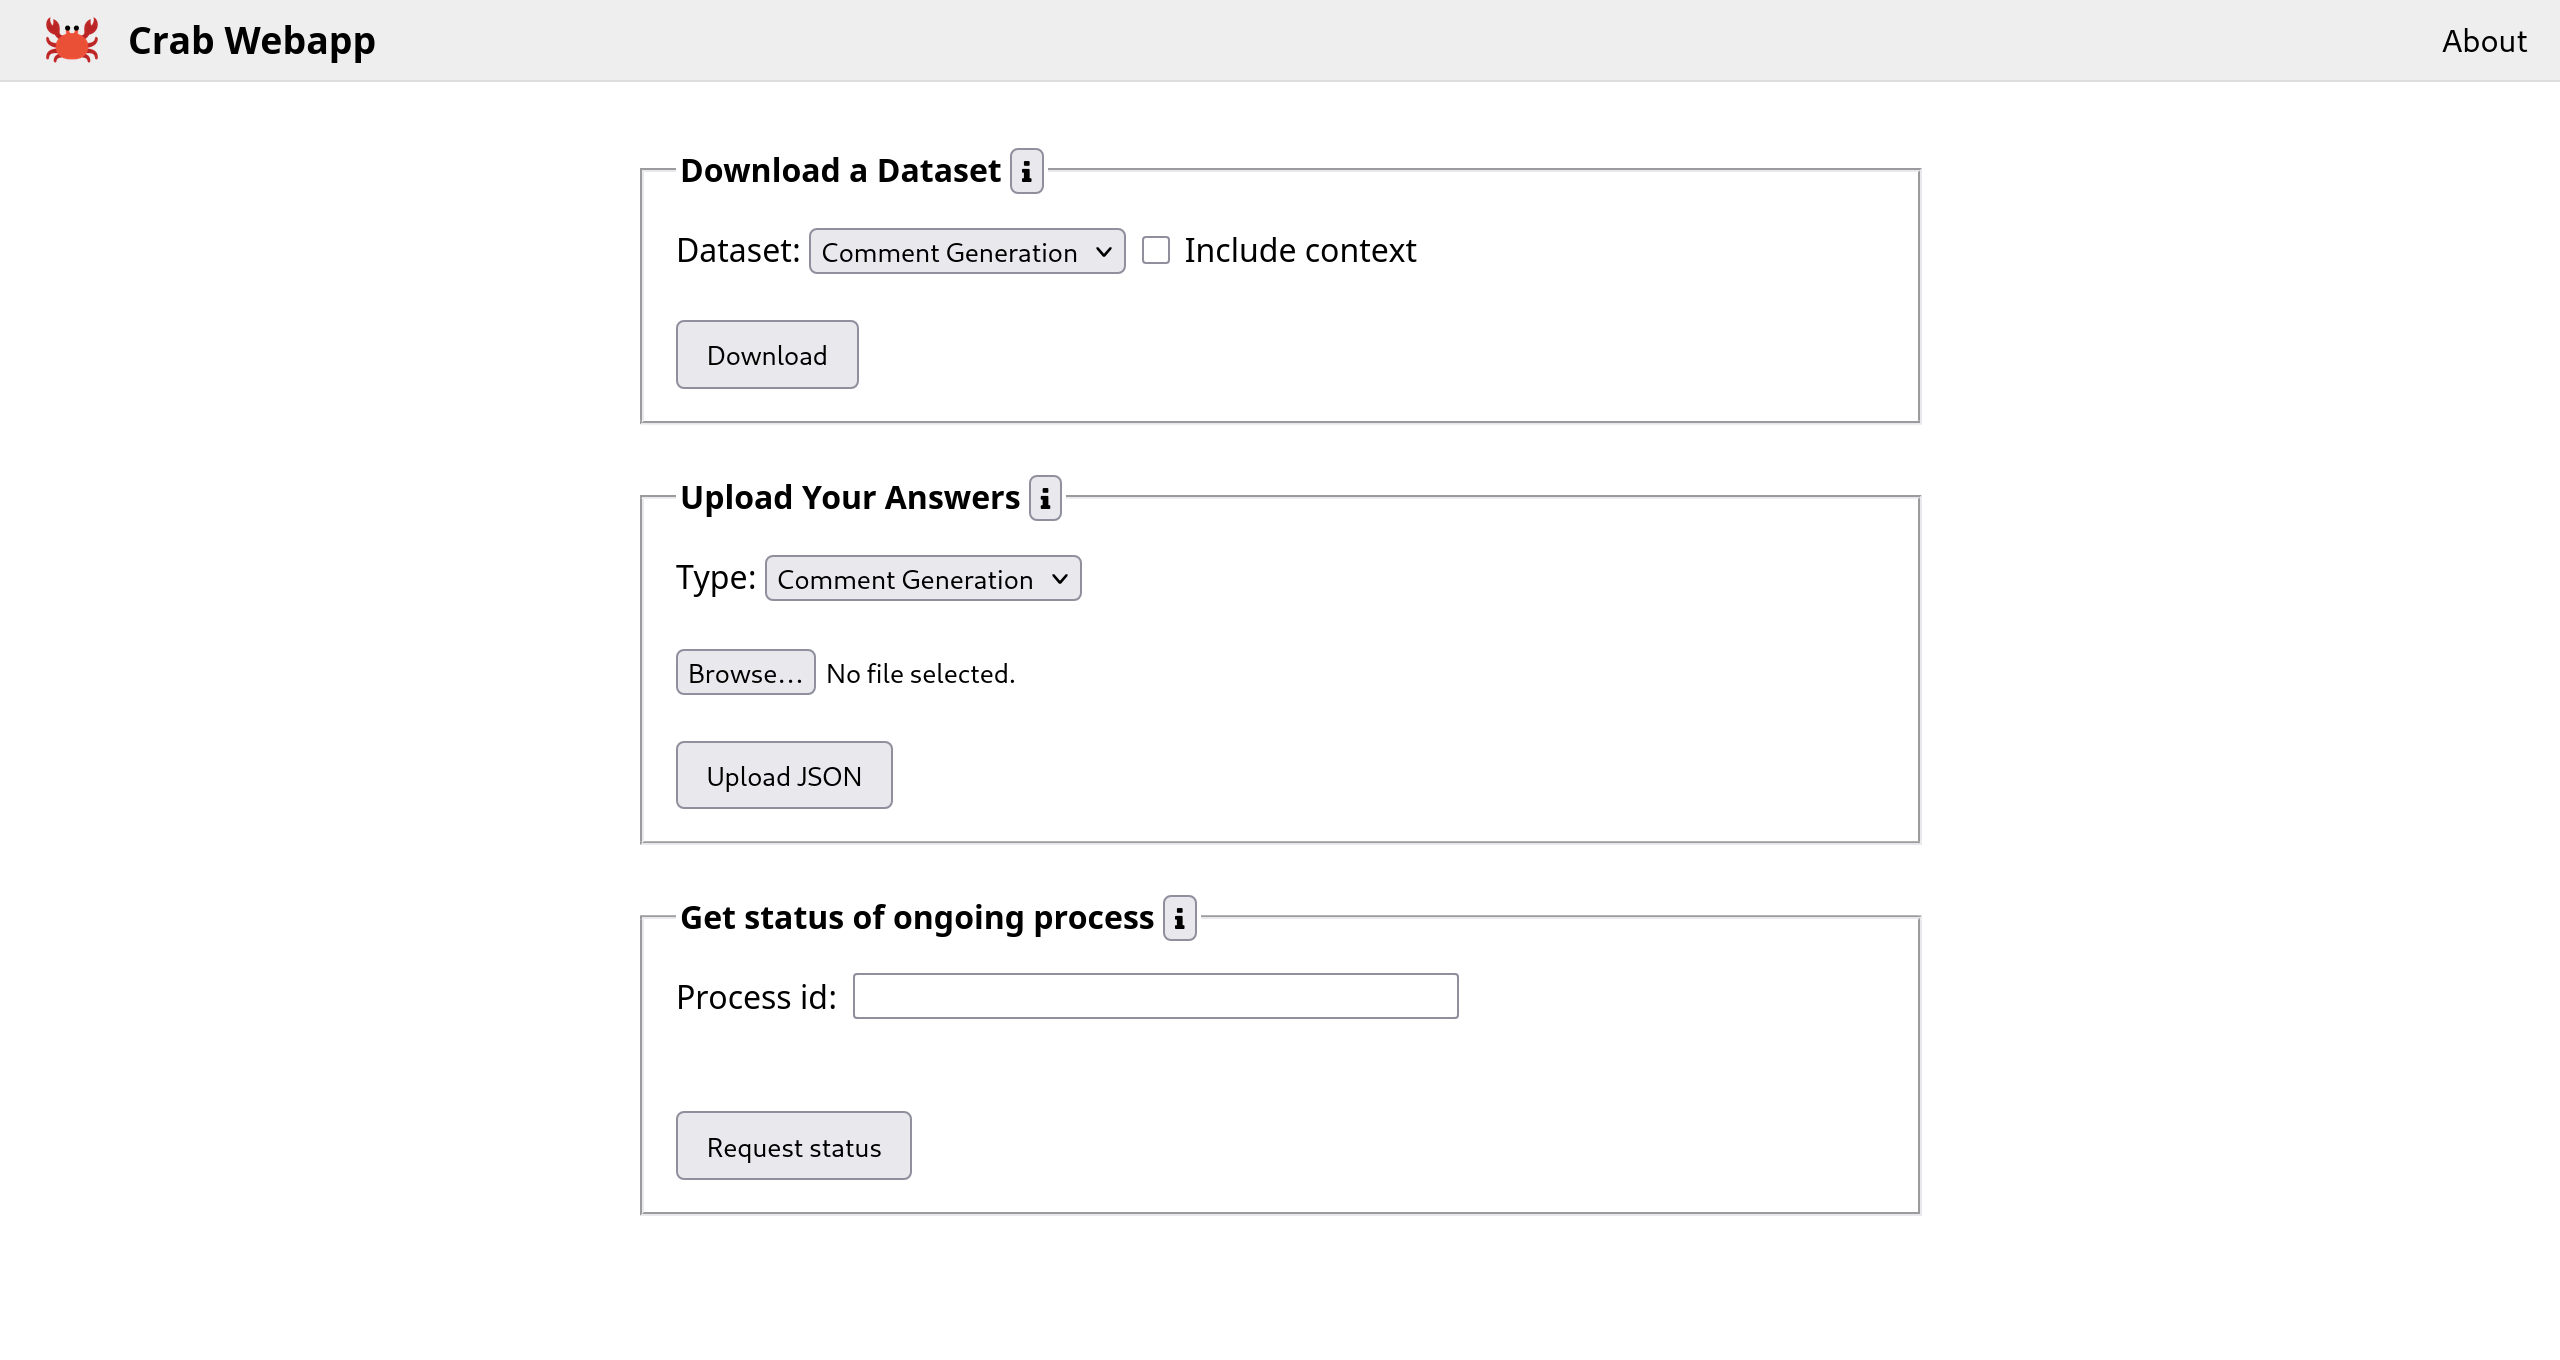
\includegraphics[width=\textwidth,cfbox=black .1pt 0pt]{entire-webiste.png}
	\caption{Main web interface with all three user-facing sections visible}
	\label{fig:full-page}
\end{figure}

The interface is divided into three main sections, each corresponding to one step in the user
workflow: downloading input data, uploading model predictions, and retrieving evaluation results, as
shown in Figure~\ref{fig:full-page}.

\paragraph{Downloading Input Data}

The first section allows users to download the input data corresponding to the benchmark tasks. A
dropdown menu enables the selection between \textit{Comment Generation} and \textit{Code
	Refinement}. Once selected, the user can download a ZIP archive containing a JSON file in the
structure described in Section~\ref{sec:req}, along with the optional repository context if
selected. The context includes the full state of the repository at the beginning of the pull
request, which can be useful for models that benefit from project-wide information.

\paragraph{Uploading Predictions}

The second section is used to upload predictions generated by the user's model. As detailed in
Section~\ref{sec:req}, submissions must follow a strict schema depending on the selected task. The
frontend ensures that the uploaded file is correctly received and passed to the backend. If the file
is well-formed, the backend responds with a unique process identifier.

\begin{figure}[H]
	\centering
	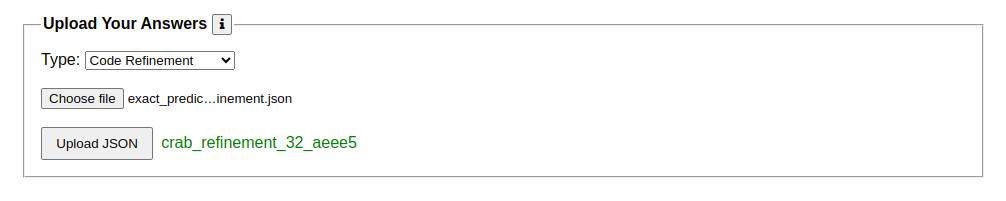
\includegraphics[width=.9\textwidth]{upload-cropped.png}
	\caption{Submission section showing the returned process ID after a successful upload}
	\label{fig:upload-id}
\end{figure}

This ID is displayed directly beside the upload button, as shown in Figure~\ref{fig:upload-id}, and
is crucial for retrieving progress updates and final results. If the user loses the ID, they lose
access to the evaluation process and its results.

\paragraph{Tracking Progress and Viewing Results}

The third section is dedicated to progress tracking and results retrieval. An input field allows
users to enter the process ID. If the user has just submitted a file, this field is pre-populated
with the returned ID. Upon submission, a live progress bar appears, indicating the current status of
the evaluation.

\begin{figure}[H]
	\centering
	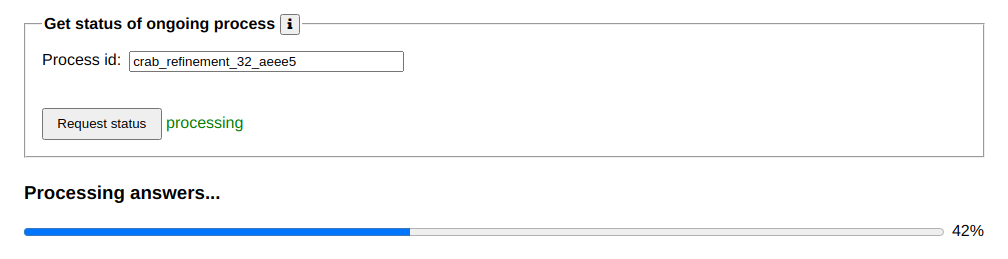
\includegraphics[width=0.9\textwidth]{progress-bar-cropped.png}
	\caption{Progress bar showing real-time status of the evaluation process}
	\label{fig:progress-bar}
\end{figure}


As illustrated in Figure~\ref{fig:progress-bar}, this feature is particularly important for the code
refinement task, where evaluation involves compiling and testing the full repository and can take
several minutes per submission. Once the process concludes, the progress bar is replaced by a
results table.

\paragraph{Comment Generation Results}

For the comment generation task, the results table includes:
\begin{itemize}
	\item The instance ID.
	\item The submitted comment.
	\item A boolean flag indicating whether the predicted comment targeted the correct file.
	\item The distance (in lines) between the predicted comment range and the original.
	\item The maximum BLEU score achieved across the original and paraphrased comments.
\end{itemize}

\begin{figure}[H]
	\centering
	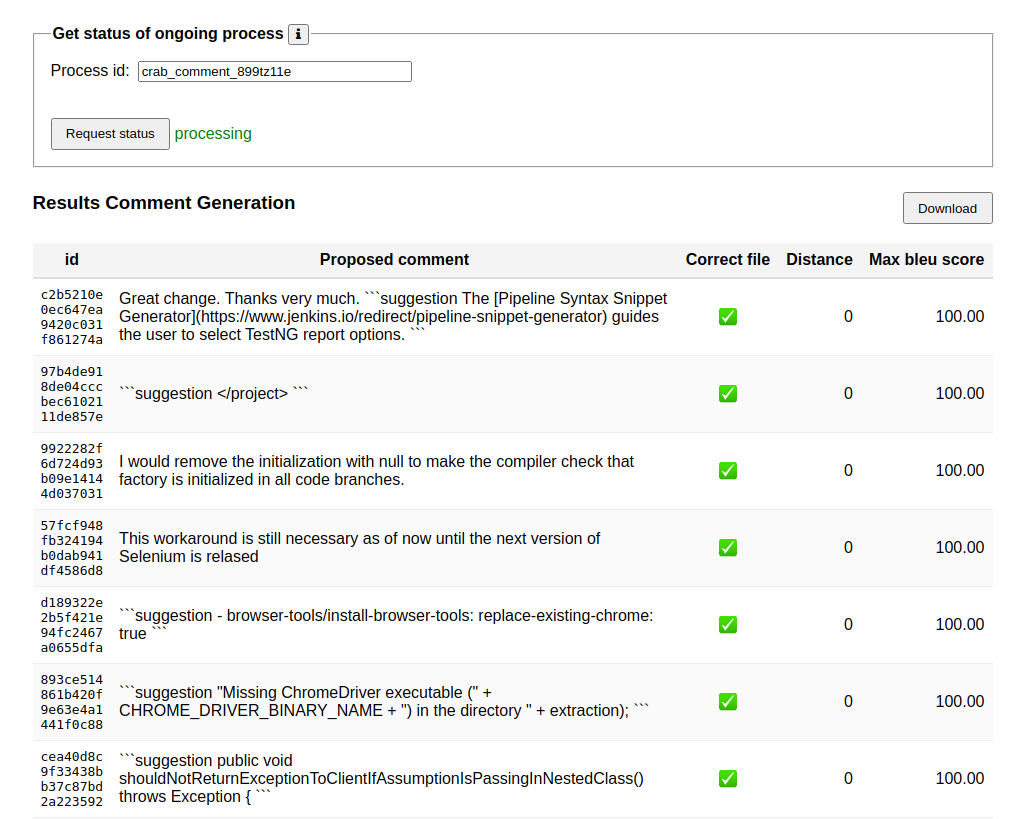
\includegraphics[width=.85\textwidth]{comment-gen-table-cropped.png}
	\caption{Result summary table for comment generation predictions}
	\label{fig:comment-table}
\end{figure}

Figure~\ref{fig:comment-table} shows the result summary. In the top-right corner of the table, a
\textit{Download Results} button allows users to retrieve the detailed evaluation. This is a JSON
file where each instance ID maps to an object containing the prediction, file correctness flag,
range distance, maximum BLEU score, and the full list of BLEU scores. As described in
Section~\ref{sec:req}, the first BLEU score corresponds to the original review comment, and the rest
to its paraphrases.

\paragraph{Code Refinement Results}

The results table for the code refinement task is more concise. It includes:
\begin{itemize}
	\item The instance ID.
	\item A boolean indicating whether compilation succeeded.
	\item A boolean indicating whether all tests passed.
\end{itemize}

\begin{figure}[H]
	\centering
	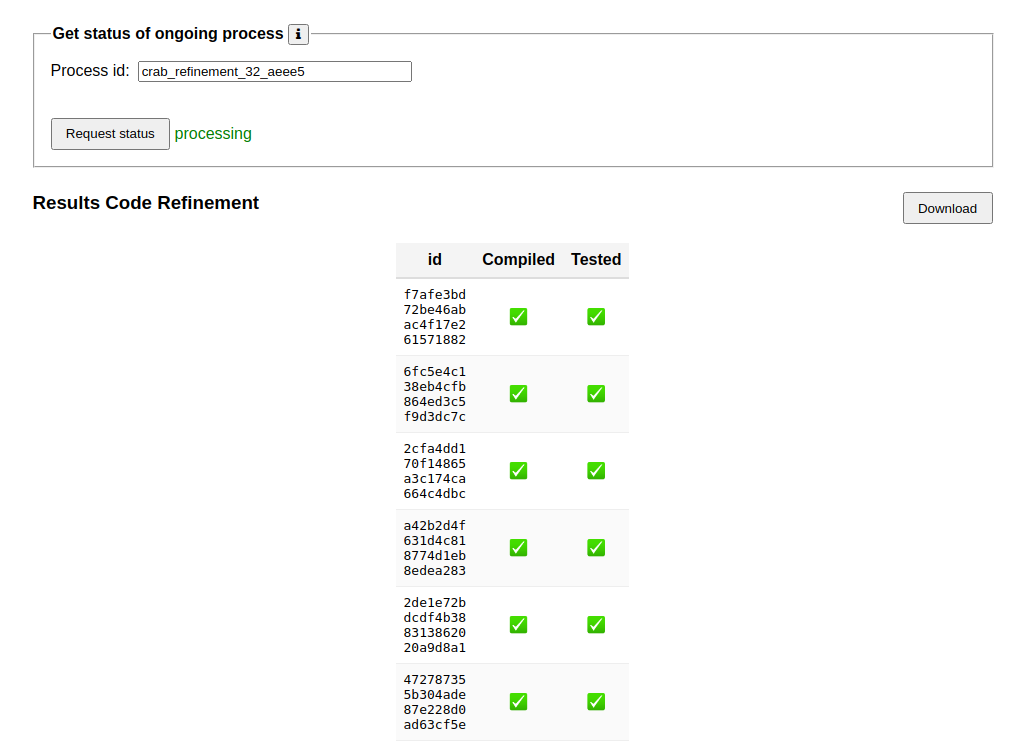
\includegraphics[width=.9\textwidth]{refinement-table-cropped.png}
	\caption{Result summary table for code refinement predictions}
	\label{fig:refinement-table}
\end{figure}

Figure~\ref{fig:refinement-table} shows the results view for this task. The downloadable detailed
results provide the same boolean indicators along with the failure messages, if any. If an instance
failed to compile, the compilation error output is included. If the tests failed, the test failure
logs are provided. This helps users quickly understand what went wrong and improve their model
accordingly.

Both results tables are fully sortable by any column. This feature enables users to quickly identify
outliers, inspect their worst- and best-performing instances, and iterate on their model behavior
efficiently.

\paragraph{User Guidance and Information Modals}

To improve usability, the interface includes several interactive help elements designed to assist
users in navigating the application without requiring external documentation. In the top-right
corner of the page (Figure~\ref{fig:full-page}), an \textit{About} button opens a modal popup
containing a high-level overview of the platform's purpose and functionality. This gives new users a
clear understanding of what the tool does and how to get started.

Each major section of the page (data download, prediction upload, and result retrieval) also
includes an information button adjacent to its title. Clicking these buttons triggers
context-specific modals that guide users through the functionality of the section. For the download
section, the modal explains the task selection process and the structure of the downloadable
dataset, including whether it includes repository context. For the upload section, users are
reminded of the required JSON structure for each task, and warned that improperly formatted
submissions will be rejected. Additionally, they are informed about the significance of the process
ID received after uploading their predictions. These modals serve as in-place documentation and
reduce user friction, especially for first-time visitors.


\subsection{Backend}

\subsubsection{Framework Choice and Migration Rationale}

The backend was originally implemented in JavaScript using the Express framework. This decision was
made based on Express’s minimal setup requirements and the widespread familiarity with JavaScript
for lightweight web servers. However, significant issues soon arose.

First, although the syntax is somewhat similar to Python, the language differences meant rewriting
some of the logic that already existed in the Python-based dataset builder. Second, and more
critically, the JavaScript ecosystem introduced reliability issues. While searching for a BLEU score
computation library, we identified a package called \path{bleu-score} \cite{bleu-score-npmjs}.
Unfortunately, the library contained bugs and had not been updated since early 2023. Rather than
rely on it, we reimplemented BLEU score computation manually to bypass the issue.

The final breaking point came during the implementation of the code refinement evaluation. To ensure
uniform results regardless of host system, we containerized the evaluation environment using Docker.
At this stage, we discovered that most Docker-related Node.js libraries were either outdated or
lacked the functionality we needed. Given these compounding issues, we abandoned Express in favor of
Flask.

Flask provided immediate benefits. The Python-based backend integrated seamlessly with existing
components from the dataset builder. More importantly, robust and well-maintained libraries were
readily available for both BLEU score computation and Docker container management. This transition
significantly reduced complexity and improved reliability.

\subsubsection{Overall Architecture}

The backend follows a modular and extensible architecture centered around the Flask web framework.
This design was chosen to promote clarity, maintainability, and seamless integration with the
Python-based tooling developed throughout the project.

At its core, the application defines an entry point that sets up the Flask server, applies CORS
policies, and registers multiple route blueprints. These blueprints group related functionality
under dedicated URL prefixes:
\begin{itemize}
	\item \path{/} and \path{/api/hello}: Health check and root endpoint, used primarily for basic
	      server diagnostics.
	\item \path{/answers}: Handles submission and status tracking for both comment generation and code
	      refinement tasks.
	\item \path{/datasets}: Provides download endpoints for the processed datasets.
\end{itemize}

A global setup step initializes the observer infrastructure (c.f. Section~\ref{sec:observer}). This
includes scanning previously stored evaluation results, cleaning up incomplete or expired entries,
and preparing the necessary directories for result caching. This ensures that even after server
restarts, previously completed evaluations can still be retrieved by ID.

Every response from the backend is formatted as JSON. This ensures the backend is easily consumable
both by browser-based clients and by external tools or scripts making programmatic HTTP requests.
This design enables seamless automation or integration with larger pipelines.

The primary user-facing endpoints are located under the \path{/answers} blueprint. This component
exposes a submission route, \path{/answers/submit/<task>}, where \path{<task>} can be either
\path{comment} or \path{refinement}, corresponding to the two main evaluation types supported.

Each submission consists of a JSON file containing either a list of proposed comments for specific
code lines (comment generation) or a mapping of filenames to their modified content (code
refinement). The backend first validates the structure of the uploaded file to ensure correctness.
If valid, it wraps the parsed data in a new \path{Subject} object and submits it to the queue
manager. The subject is assigned a unique ID and saved in an in-memory mapping for future access.

Clients are provided with a URL pointing to \path{/answers/status/<id>}, where they can poll for
updates or retrieve the final result once evaluation has completed. Optionally, a WebSocket
connection can be established by the client using a unique socket identifier. This allows the
backend to register a corresponding \path{SocketObserver} that receives live updates as the task
progresses. If the client disconnects, its observer is unregistered to free resources.

The backend maintains strict separation between task execution and client interaction. Evaluation
functions such as BLEU score computation or Docker-based testing are functions that are completely
agnostic of what surrounds them, they report their progress only via callback mechanisms. The
subject object intercepts these callbacks and translates them into observer notifications or status
updates.

To summarize, the architecture consists of:
\begin{enumerate}
	\item A clean separation of concerns between routing, task execution, and client communication.
	\item A subject-observer system enabling real-time progress tracking with on-demand observer
	      registration.
	\item A thread-pooled queue manager that ensures controlled parallelism and consistent resource
	      usage.
	\item Persistent result caching that allows evaluation results to survive restarts and be reused
	      or inspected later.
\end{enumerate}

This setup provides a robust backend that supports asynchronous, real-time task evaluation in a
scalable and modular fashion.


\subsubsection{Observer Pattern and Queue Management}
\label{sec:observer}

A central requirement for the backend was the ability to track the progress of submitted tasks in
real time, with support for multiple clients observing the same process from different devices or
sessions. The solution to this challenge emerged naturally through the application of the observer
design pattern.

The observer pattern was implemented via two core abstractions: \path{Subject} and
\path{Observer}. Each \path{Subject} represents a single evaluation task, either comment
generation or code refinement. The \path{Observer} interface defines three callback
methods: \path{updateStarted}, \path{updatePercentage}, and \path{updateComplete}, which are
used to propagate state changes to registered observers. Concrete implementations of
\path{Observer}, such as \path{SocketObserver}, encapsulate communication channels like
WebSocket clients and use these callbacks to relay updates.

Upon submission, a new subject is created and immediately associated with a unique identifier. This
subject encapsulates the evaluation function as a callable, along with two internal callbacks: one
for progress reporting and one for completion. Crucially, the evaluation logic is designed to be
agnostic of its context: it does not concern itself with how the results are used or who is watching.
It simply calls the progress and completion callbacks with appropriate values.

The subject, in turn, translates these callbacks into observer notifications. When the task starts,
all registered observers are informed. As progress is made (e.g., per-item BLEU score computation or
per-step refinement testing), percentage updates are broadcast. When the task concludes, each
observer receives a final result payload. These interactions are fully decoupled: observers can join
or leave at any time without affecting the execution of the task.

This flexible observer design allows late-joining clients to attach to ongoing processes and still
receive meaningful updates. For example, if a subject is in the \path{PROCESSING} state, a newly
registered observer will immediately be informed of the current progress percentage. If the subject
has already completed, the result is returned directly without even registering the observer, as no
further updates are necessary. Observers are explicitly unregistered once they receive final results
to avoid memory leaks and stale references.

To handle concurrency, a custom queue management system wraps the subjects and regulates their
execution lifecycle. Submitting a subject to the backend does not trigger immediate execution.
Instead, the subject is placed into a first-in-first-out queue managed by the \path{QueueManager}
class. This manager uses Python’s \path{ThreadPoolExecutor} to cap the number of concurrently
running evaluations, ensuring the system remains responsive and resource-safe.

Each subject transitions through a well-defined state machine:
\begin{itemize}
	\item \path{CREATED}: The subject has been initialized but not yet enqueued.
	\item \path{WAITING}: The subject is in the queue, waiting for an available execution thread.
	\item \path{PROCESSING}: The task is actively running in a thread.
	\item \path{COMPLETE}: The task has finished and the results are available.
\end{itemize}

When a subject enters the \path{WAITING} state, its position in the queue can be queried via the
WebSocket interface or the HTTP status endpoint. This is particularly useful for long queues, as it
allows users to anticipate when their task will begin. Once a thread becomes available, the subject
is dequeued, transitions to \path{PROCESSING}, and its task is executed. Progress updates are
issued as the evaluation proceeds, eventually culminating in a state change to \path{COMPLETE} and
the caching of final results.

The final design elegantly decouples task execution, progress tracking, and client communication. It
allows real-time observability of complex processes while maintaining modularity and robustness. By
separating concerns and embracing well-established design patterns, the system remains scalable and
adaptable to future changes, such as the introduction of new evaluation types or alternative
notification mechanisms.


\subsubsection{Paraphrase Evaluation Pipeline}
\label{sec:paraphrases-check}

The paraphrase evaluation pipeline processes submissions aimed at generating natural language
comments describing a code change. Each submission is a proposed comment intended to annotate a
specific line range in a given file. The evaluation is designed to measure both the semantic
similarity of the submission to a ground-truth comment and the contextual relevance of its placement
in the code.

Upon receiving a submission, the backend first matches it against the corresponding reference entry
in the dataset using the provided identifier. The system then compares the proposed comment to a set
of target comments associated with that dataset entry. This set includes the original human-written
comment as well as a number of paraphrases generated during the dataset construction phase.

The primary metric used is the BLEU score, a well-known automatic evaluation metric in natural
language processing. For each target paraphrase, the BLEU score is computed against the proposed
comment. The final result includes:
\begin{itemize}
	\item The highest BLEU score across all references.
	\item The list of individual BLEU scores per paraphrase.
	\item The original comment submission for traceability.
	\item A binary flag indicating whether the submission was made on the correct file.
	\item A distance metric estimating how close the submitted line range is to the target line range.
\end{itemize}

This evaluation is executed entirely within the Python backend using the \path{sacrebleu} library
\cite{sacre-bleu}.
As the evaluation proceeds, a percentage indicator is updated and used to notify any observers via
the subject-notification infrastructure described earlier. Upon completion, results are returned
either through polling or via WebSocket push notification.

\subsubsection{Code Refinement Evaluation Pipeline}
\label{sec:refinement}

The code refinement evaluation pipeline processes submissions where users attempt to fix or improve
code by modifying one or more files. These modifications are evaluated in a reproducible environment
using Docker-based containerization to ensure consistency across machines and platforms.

Each submission consists of a mapping from filenames to updated file contents. When the backend
receives a submission, it identifies the corresponding dataset entry and retrieves the associated
project archive. The archive captures the exact state of the repository at the moment the pull
request was merged, ensuring that evaluations are performed on the finalized version of the code.

The evaluation process proceeds through the following steps:
\begin{enumerate}
	\item A build handler is initialized for the project, tailored to its build system.
	\item The proposed file changes are injected into the local copy of the project.
	\item The modified project is compiled to ensure that the changes do not introduce syntax or build
	      errors.
	\item If compilation is successful, the project’s test suite is executed to validate the
	      functional correctness of the changes.
\end{enumerate}

At each step, any failure is recorded along with an error message, and the evaluation for that
submission is halted. Successful evaluations result in a dictionary that indicates the status of
each step: file injection, compilation, and testing.

Similar to the comment generation flow, the refinement evaluation uses progress callbacks to emit
state updates to observers. A rough percentage is calculated based on progress through the four
discrete steps: initialization, injection, compilation, and testing. Final results are cached and
made available to the client once the evaluation concludes.

This pipeline ensures fairness and reproducibility by isolating each evaluation in a controlled
environment, thereby avoiding inconsistencies caused by external system dependencies or
configuration mismatches.


\section{Conclusions and Future Work}

In this work, we have successfully attained our primary goal of creating a rigorously curated
dataset of code review instances. After manual selection and validation, our comment generation
dataset comprises 894 high-quality instances, and our code refinement dataset comprises 57
instances. While we would have wished for a larger code refinement set, we have laid the groundwork
for future efforts to improve upon this number.

As noted in Sections \ref{sec:stat-small} and \ref{sec:stat-expanded}, these figures derive from an
initial pre‐filtering of repositories: only 398 out of 4'795 total projects were retained because
their latest commit used a supported build system (Maven or Gradle), compiled, and passed at least
one test. This filter, while ensuring immediate reproducibility, significantly limits the scope of
our corpus. Across all repositories, just 0.32\% of pull requests qualified for the code refinement
task, versus 7.61\% within the pre‐filtered set; conversely, we uncovered 16'376 candidate PRs for
comment generation in the full corpus (versus 1'704 pre‐filtered). Importantly, we halted the
full-corpus pipeline after ten days of execution,processing roughly 300 projects, to inspect
intermediate results, so the 16'376 figure is a lower bound and additional eligible PRs likely
remain undiscovered. A promising avenue to boost code refinement instances would be to relax the
``last-commit builds and tests'' requirement: by only enforcing build-system support and the presence
of tests, we could include many more repositories while still guaranteeing that PRs culminate in a
compilable, testable state.

As discussed in Sections \ref{sec:pr-selection} and \ref{sec:dataset-download}, another enhancement
would be to accommodate pull requests with multiple reviewer comments. This would require
attributing each review‐induced code change to its corresponding comment, thereby generating
multiple valid triplets per PR. Disentangling interleaved comments and overlapping edits poses a
complex annotation challenge, but our tool's modular, containerized, and reproducible architecture
is well suited to incorporate such extensions without major rework.

On the tooling side, we fully implemented the benchmarking framework via our web application, which
supports both comment generation and code refinement tasks.  Thanks to the language‐agnostic design
of both the data‐construction pipeline and the webapp (Section \ref{sec:exec-env}), the system can
compile, test, and evaluate submissions in any language or build system with minimal additional
configuration.  This architecture ensures independent, containerized execution of each job, proof of
its robustness and ease of extension to new ecosystems, and the integrated queuing system provides
real‐time progress updates with minimal resource overhead.  Users can submit jobs, monitor results,
and depart at will, enabling horizontal scaling to accommodate large numbers of concurrent
evaluations while preserving administrative control under heavy load.  Future work could thus focus
on adding out‐of‐the‐box support for languages beyond Java (e.g., Python, JavaScript, C++),
broadening the benchmark's applicability.

Although it was our initial plan to benchmark the performance of current state‐of‐the‐art models
against our dataset, time constraints imposed by thesis deadlines prevented us from doing so. Such
experiments would yield valuable insights into where our benchmark sits within the landscape of
automated code review research, and would help identify practical improvements, both to the webapp's
evaluation pipelines and to our dataset construction methodology. Importantly, there are no
technical barriers preventing this assessment: both dataset and tool are fully functional and
readily available. We therefore strongly encourage future users to leverage our dataset and
benchmark platform to evaluate leading models, publish comparative results, and drive further
advances in automated code review.

In closing, this thesis contributes a novel, high‐quality benchmark and a flexible evaluation tool
that together establish a solid empirical foundation for the development of next‐generation code
review automation. By providing both curated data and an extensible evaluation environment, we hope
to accelerate research in comment generation and code refinement, and to inspire future work that
pushes the boundaries of automated software quality assurance.



\newpage
\bibliographystyle{unsrt}
\bibliography{biblio}

\end{document}
